\chapter{Background Estimation}
\label{chap:bkg}

Due to the lifetime ($c\tau > 2$ mm) and mass ($m > 10$ GeV) requirements applied at vertex selection, no SM background is expected in the signal region in search for displaced dilepton resonance. Therefore, two non-collision backgrounds are considered in this search: cosmic background and \textit{random-crossing} background. The cosmic background is the dominant background in this analysis and is estimated In Section~\ref{sec:bkg:cosmic}. In Section~\ref{sec:bkg:random}, background from random-crossing of two uncorrelated tracks are estimated.


\section{Cosmic Background}
\label{sec:bkg:cosmic}

A cosmic muon passing through the ID during a collision event can be reconstructed as a back-to-back muon pair with opposite electric charges, and the pair can be reconstructed as a displaced \mumu vertex passing all signal selection criteria in this analysis. \mumu vertex.

This cosmic background is suppressed by implementing the cosmic veto, $R_{\mathrm{CR}} < 0.01$ (Section~\ref{sec:event_selection}). The event cut flow in Figure~\ref{subfig:event_cutflow_MC} shows that the cosmic veto is very effective in signal selection, i.e., the signal efficiency loss due to the cosmic veto is negligible. To illustrate the $R_{\mathrm{CR}}$ distribution of cosmic muons, a cosmic control region is defined as follows:

\begin{itemize}
  \item Events are required to fail the cosmic veto.
  \item Events are required to have at least two muons satisfying vertex track selection (Table~\ref{table:vertex_track_selection_simple}).
  \item All other event selections are kept the same as the signal region.
\end{itemize}

In this control region, pairs of two muons with leading $p_{T}$ are studied using the data sample. Figure~\ref{fig:cosmicData} shows the distribution of the pairs in $|\Delta\phi|$ and $\Sigma \eta$. The distribution shows that a significant faction of muons pairs is from cosmic rays and is constraint in small $R_{\mathrm{CR}}$ region.

\begin{figure}[!htb]
    \begin{center}
    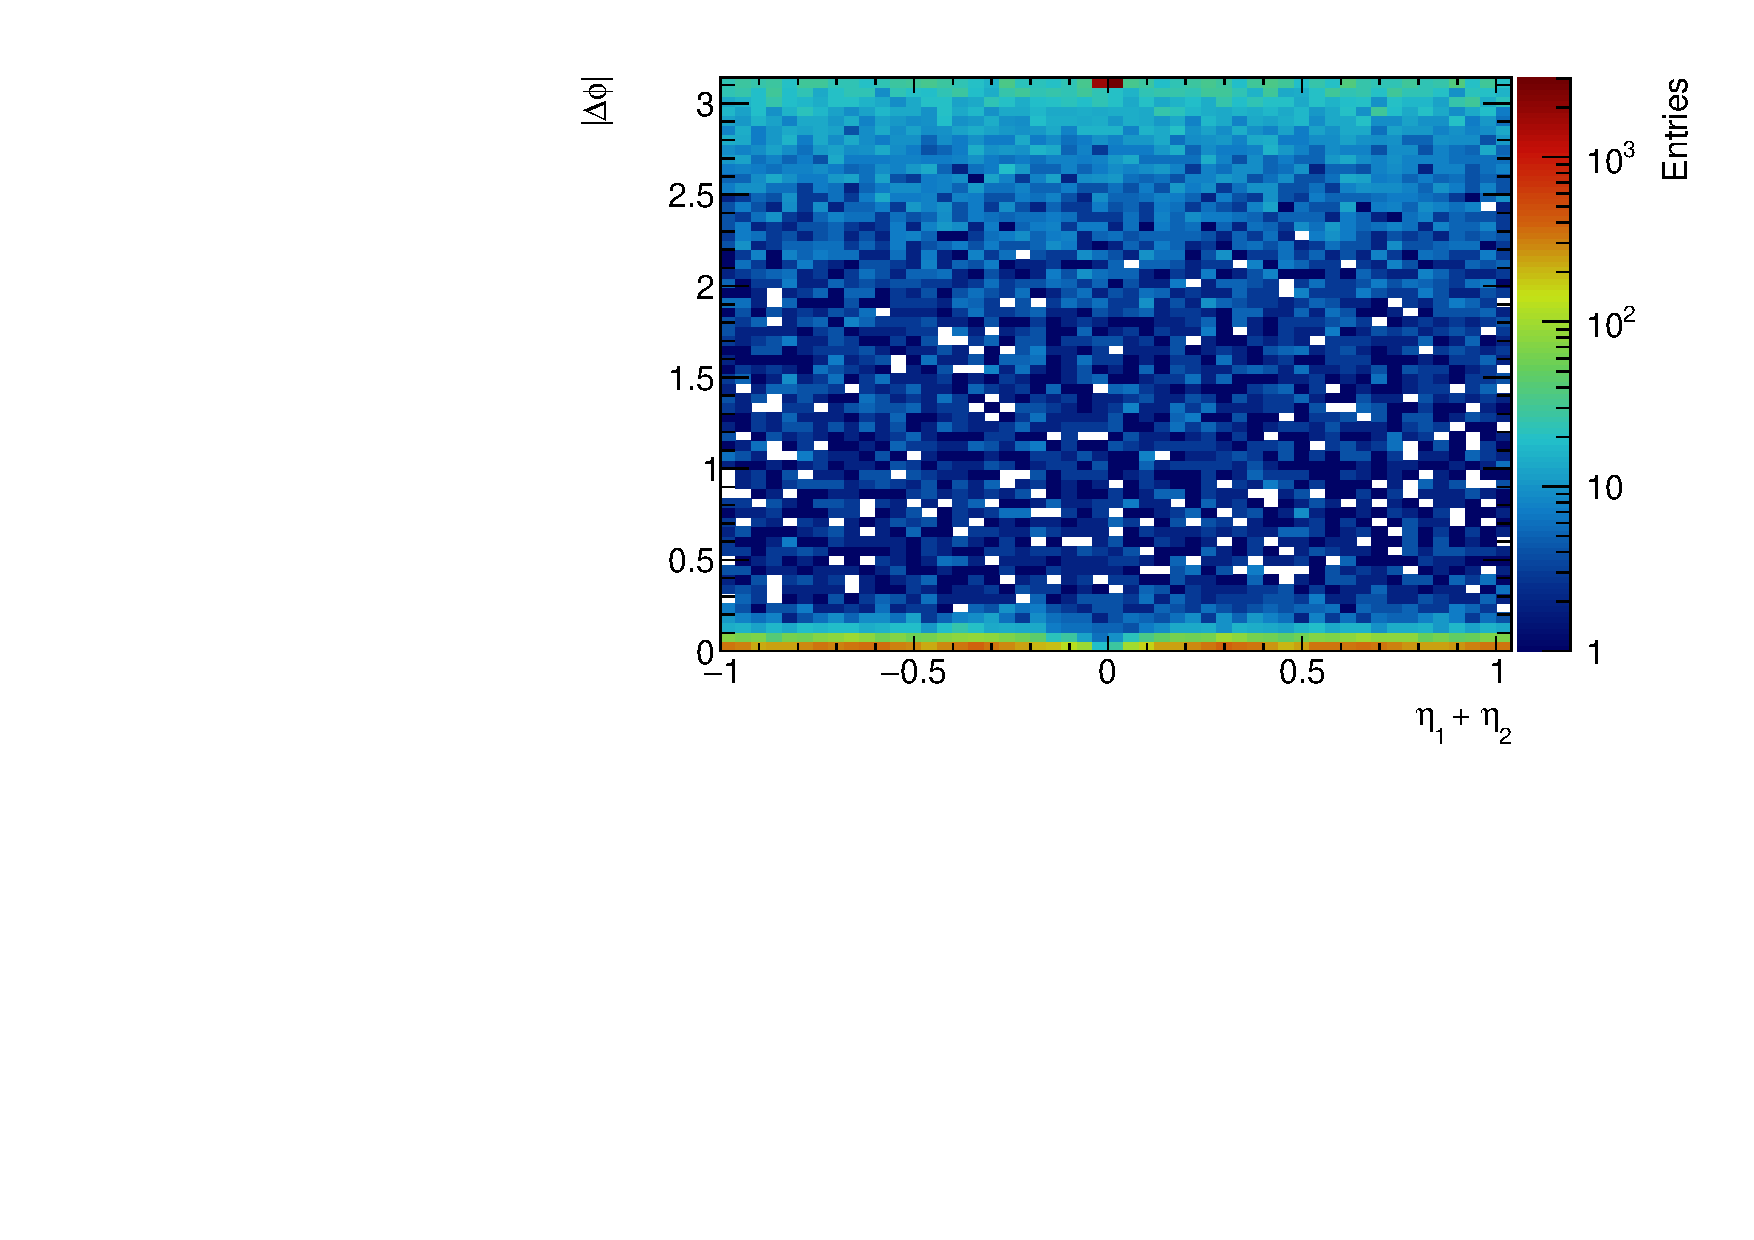
\includegraphics[width=0.6\textwidth]{figures/Cosmics/DataValidation/mup_seta_dphi.pdf}
    \label{fig:cosmicData}
    \caption{Distribution of pairs of two muons with leading $p_{T}$ in $|\Delta \phi|$ and $\Sigma \eta$ found in the cosmic control region using the data sample. The sharp peak at $|\Delta\phi| = \pi$ and $\Sigma \eta = 0$ shows that a significant fraction of muon pairs in the region is from cosmic muons.}
\end{center}
\end{figure}

To estimate the cosmic background in the signal region, the distributions of \mumu vertices and pairs from the data sample in small $R_{\mathrm{CR}}$ region are shown in Figure~\ref{fig:cosmicCR}. There are 246 \mumu vertices found in the data sample that pass all of the signal selection except the cosmic veto, and the distribution vanishes around $R_{\mathrm{CR}}=0.004$\mumu, suggesting that the cosmic background is effectively suppressed by the cosmic veto cut of $R_{\mathrm{CR}}=0.01$.

For more accurate estimation of the background, the \mumu pair distribution is normalized to the \mumu vertex distribution as shown in Figure~\ref{fig:cosmicCRb}, and the normalized distribution is extrapolated to the signal region. With this method, the cosmic background is estimated to be 0.27$\pm$0.14 (stat.). This background is about two
orders of magnitude larger than the random crossing background. Therefore, the cosmic muon background is the dominant source of background for this analysis.


\begin{figure}[!htb]
    \centering
    \subfloat[Unscaled\label{fig:cosmicCRa}]{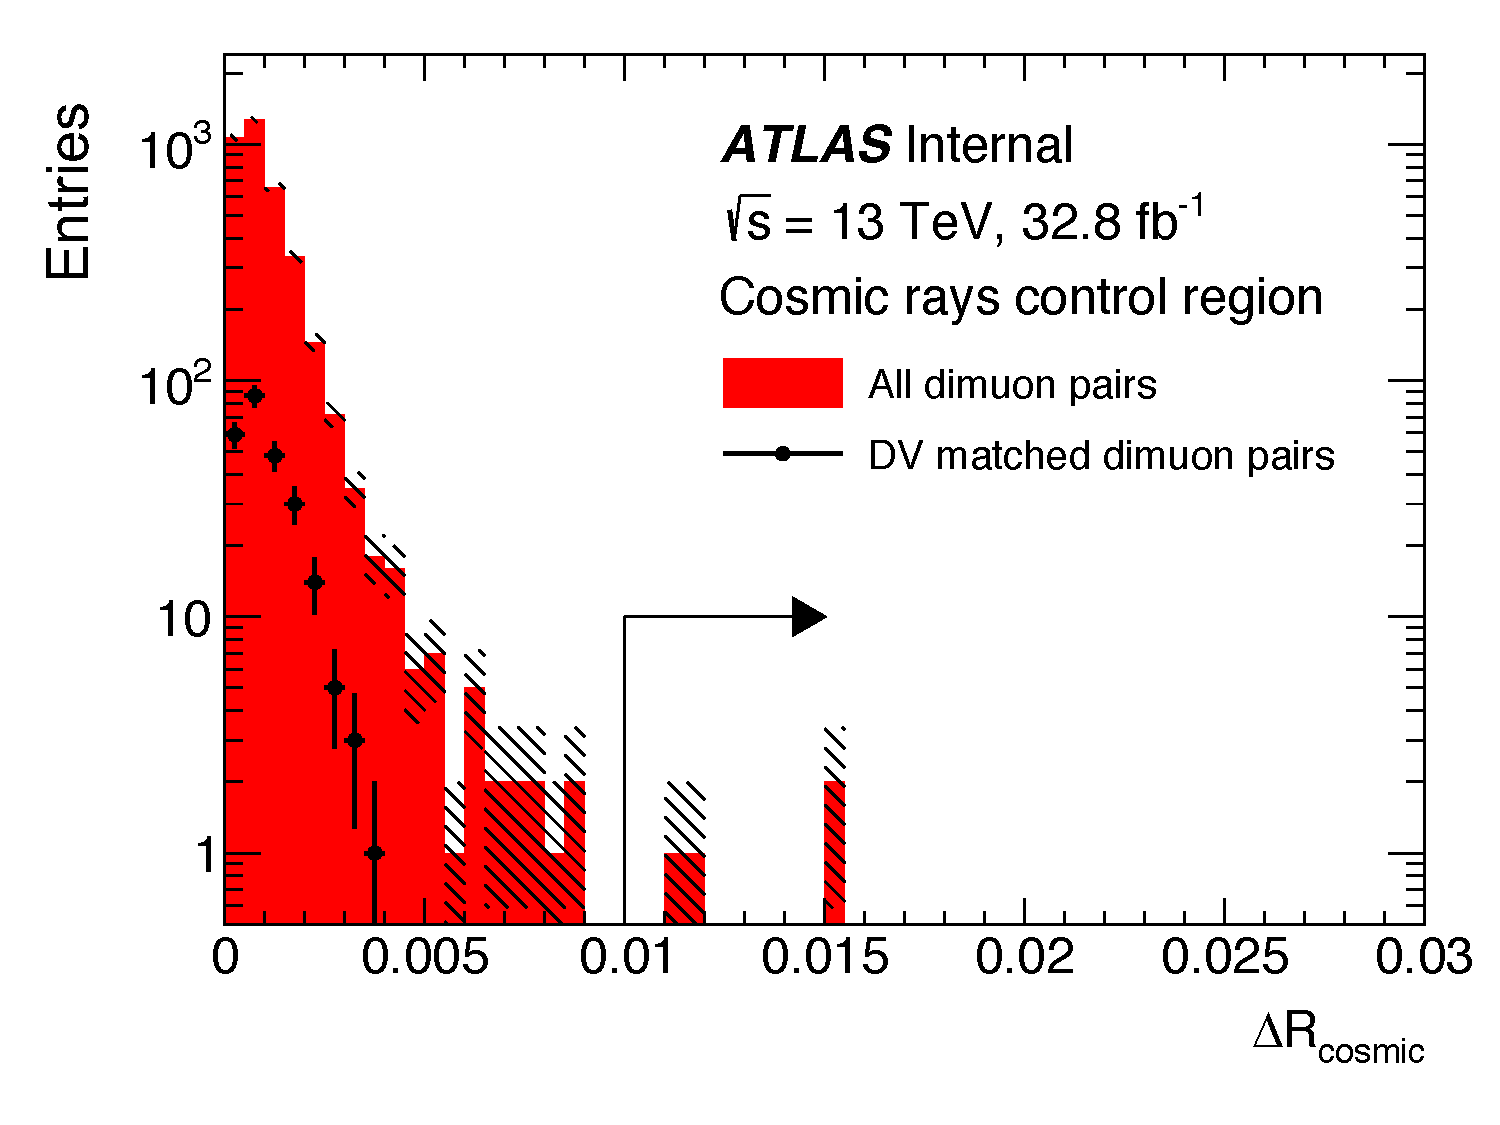
\includegraphics[width = 0.49 \textwidth]{figures/Cosmics/DataValidation/cosmics_unscaled.pdf}}
    \subfloat[Scaled\label{fig:cosmicCRb}]{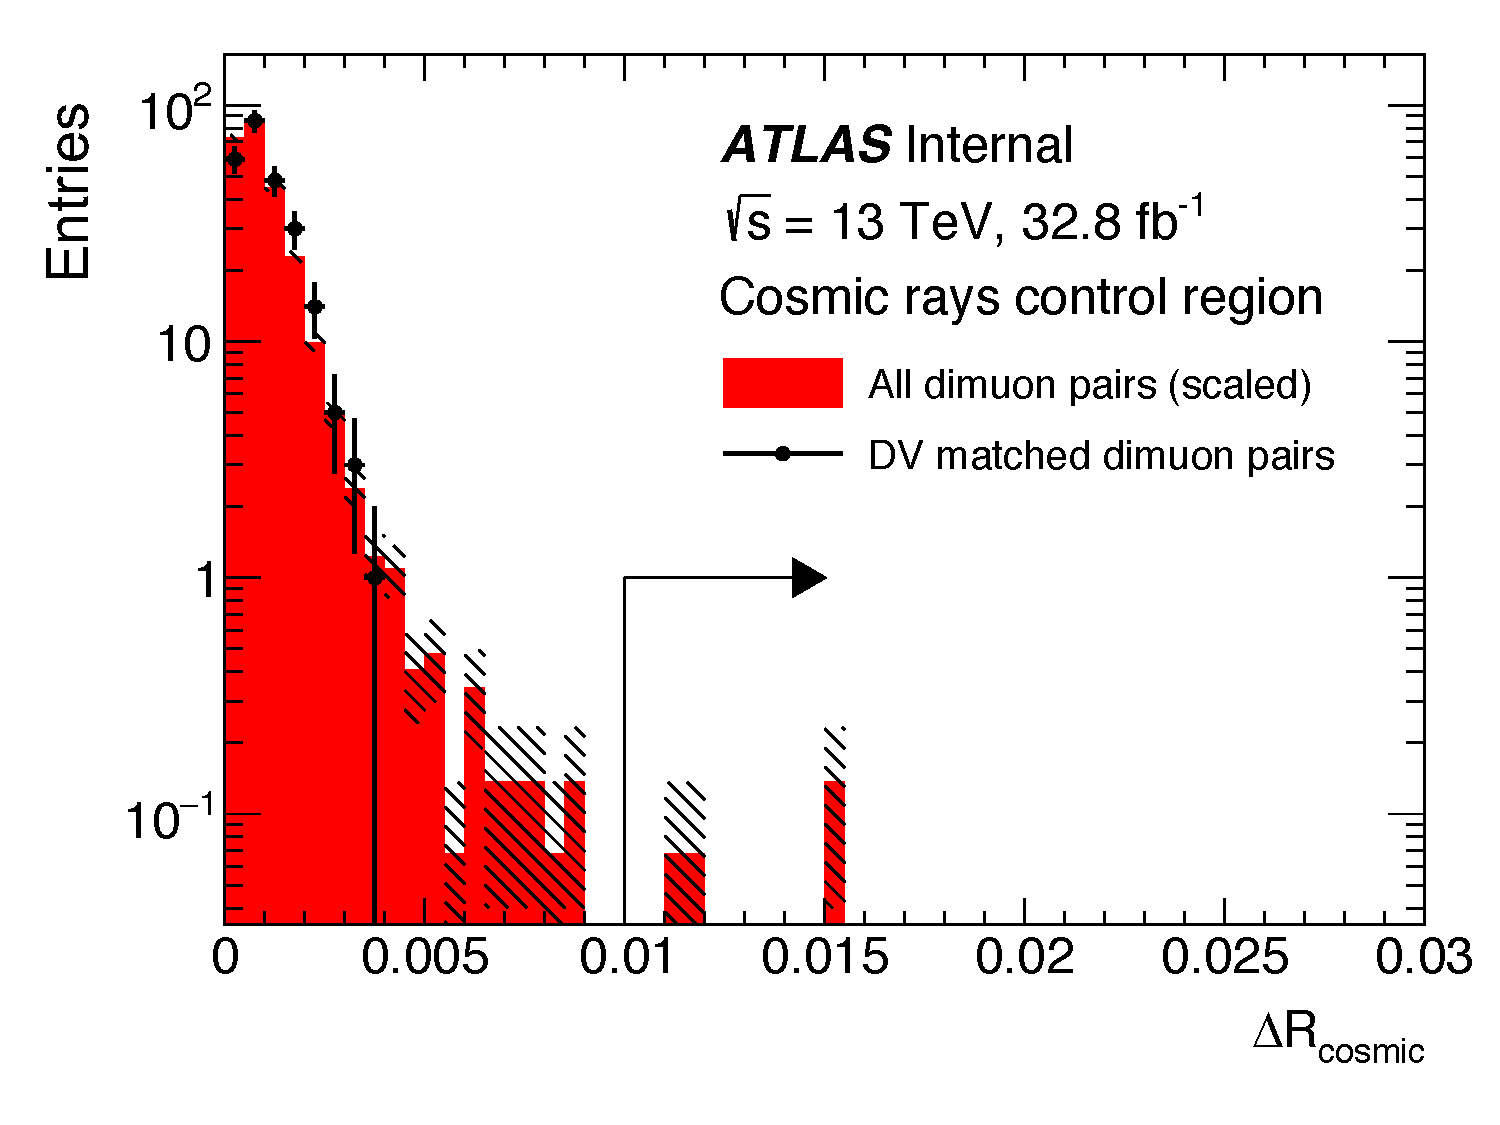
\includegraphics[width = 0.49 \textwidth]{figures/Cosmics/DataValidation/cosmics_scaled.pdf}}
    \label{fig:cosmicCR} 
	\caption{(a) Distribution of \mumu vertices and pairs from the data sample in small $R_{\mathrm{CR}}$ region. The red distribution represents all \mumu pairs. The black dots represent the subset of pairs forming a \mumu vertex. The same distribution is shown in (b) with \mumu pairs normalized to \mumu vertices.}
\end{figure}



\section{Random-Crossing Background}
\label{sec:bkg:random}

The random-crossing of two uncorrelated tracks can be a major source of the backgrounds in the search for displaced dilepton vertices. This background is expected to increase with more pile up in Run 2.
 
This random-crossing background is estimated by a data-driven method called the \textit{track flipping} (TF). In this method, secondary vertex reconstruction is performed on each pair of tracks from all possible combinations of tracks after one random track from each pair is flipped with respect to the beam spot. Because one track is flipped in each pair of tracks, the resulting vertices provide good estimation for random-crossing background. In addition, another random-crossing background method called the \textit{Event mixing} is used to estimate systematic uncertainty in the background estimation.

The TF and event mixing methods are described in Section~\ref{sec:bkg:random_crossing_tf} and ~\ref{sec:bkg:random_crossing_em}, respectively. In Section~\ref{sec:bkg:random_crossing_MC}, the TF method is tested on the background MC samples, and the result is compared with the corresponding result from the event mixing. In Section~\ref{sec:bkg:random_crossing_data}, the random-crossing background in data is estimated by the TF method.%, and its systematic uncertainty is estimated by comparing the estimation from the TF and event mixing in Section~\ref{sec:bkg:random_crossing_syst}.

\subsection{Track Flipping Method}
\label{sec:bkg:random_crossing_tf}

In the TF method, events are selected by the same requirement described in Section~\ref{sec:selection:pre}. From the selected events, ID tracks associated with a muon, electron, or neither, referred as muon, electron, or non-leptonic track, respectively, are selected with the track criteria (Table~\ref{table:vertex_track_selection_simple}) used for the secondary vertexing algorithm. Lepton tracks are required to pass the same selection criteria described in Table~\ref{table:lepton_requirement}. Non-leptonic tracks are required to pass the minimal kinematic selection ($p_{T} > 10$ GeV, $\eta < $2.5 to match with the kinematic selection for leptons.

\begin{figure}[!htb]
    \subfloat[]{\label{subfig:TF_diagram_a}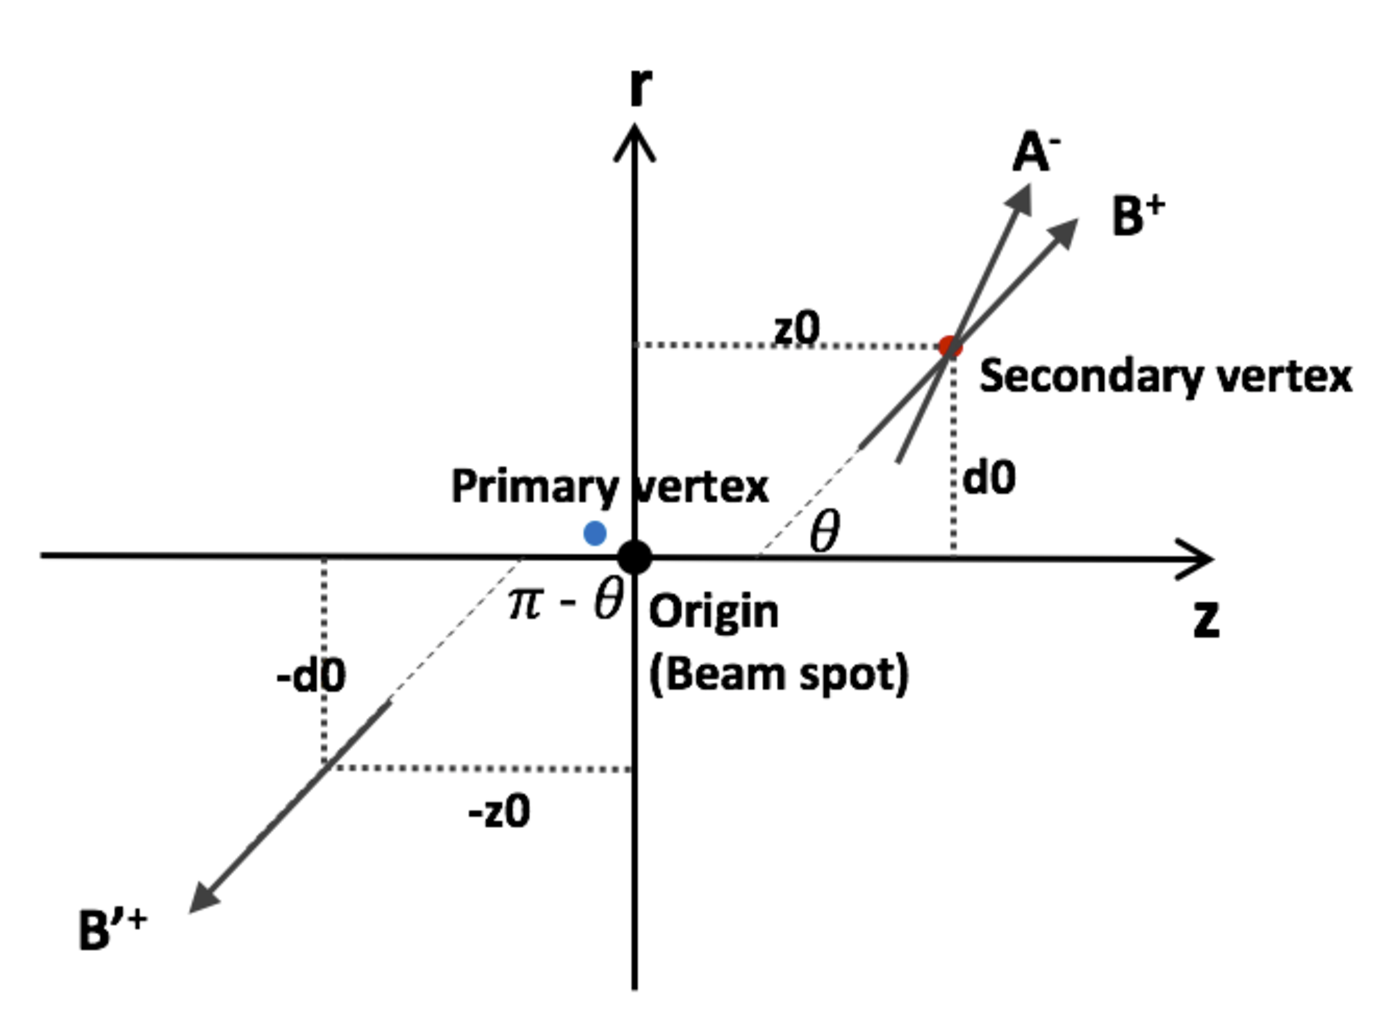
\includegraphics[width=0.50\textwidth]{figures/TF_diagram_a.pdf}}
    \subfloat[]{\label{subfig:TF_diagram_a}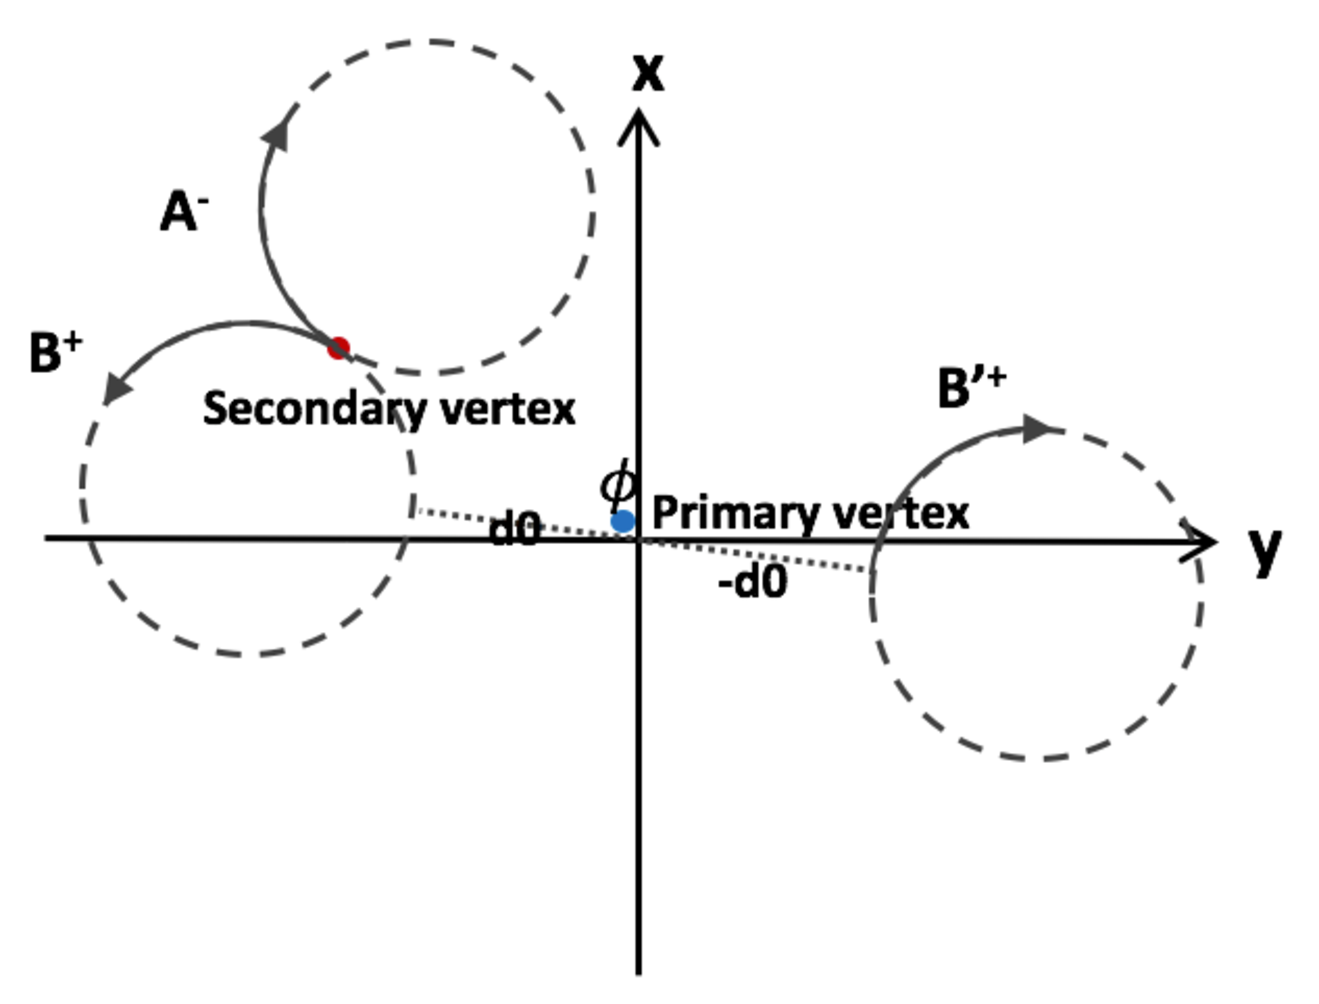
\includegraphics[width=0.50\textwidth]{figures/TF_diagram_b.pdf}}
	\centering
	\caption{Description of track flipping method in (a) $r-z$ and (b) $x-y$ plane. Given two tracks $A$ and $B$ originating from a common secondary vertex, one random track is flipped with respect to the beam spot and is denoted as $B'$. The resulting flipped track pair, $AB'$, cannot form a vertex due to the separation in space.}
	\label{fig:TF_diagram}
\end{figure}

From the selected tracks, track pairs are created from all possible combination of muon, electron, or non-leptonic tracks which fall into one of the six categories, \mumu, \ee, \emu, \ex, \mux, or \xx track pair, where x represents a non-leptonic track. For each pair of tracks, one random track is flipped with respect to the beam spot ($\dzero \rightarrow -\dzero, \zzero \rightarrow -\zzero, \phi\rightarrow\phi+\pi, \theta\rightarrow\pi-\theta$), creating a \textit{flipped track pair}. The secondary vertex algorithm used in the reconstruction of data or MC sample is used to reconstruct displaced vertices using these flipped track pairs. Vertex selection cuts similar to the cuts listed in Table~\ref{table:vertex_track_selection_simple} are applied to the vertices found from flipped track pairs. The only differences in the vertex cuts are:

\begin{itemize}
\item Trigger matching is only required for \mumu, \ee, and \emu vertices because non-leptonic tracks cannot be matched to lepton triggers, 
\item Filter matching is only required for \mumu, \ee, and \emu vertices for the same reason.
\end{itemize}

The resulting vertices, referred as \textit{track-flipping vertices}, fall into one of the same six categories as track pairs. Because one random track is flipped, track-flipping vertices are purely from random-crossing of tracks as depicted in Figure~\ref{fig:TF_diagram}. Therefore, track-flipping vertex yields provide a good estimation for random-crossing background of each type. Also, because trigger and filter matchings are not required in the control and validation region, the TF method provides conservative background estimation. 



\subsection{Event Mixing Method}
\label{sec:bkg:random_crossing_em}

The event mixing method is similar to the TF, but instead of flipping a track from pair of tracks, it combines tracks from different events to create uncorrelated track pairs, i.e., two tracks are not originating from a real vertex.

The event mixing method proceed as follows. First, muon, electron, and non-leptonic tracks that satisfy the track criteria (Table~\ref{table:vertex_track_selection_simple}) are collected from all events, resulting in a collection of all potential seed objects in the sample. Lepton tracks are required to pass the same selection criteria\footnote{Only lepton pairs with an invariant mass greater than $6~\si{\GeV}$ are used in the normalization procedure to remove any contamination from low mass processes.} described in Table~\ref{table:lepton_requirement}. Non-leptonic tracks are required to pass the minimal kinematic selection ($p_{T} > 10$ GeV, $\eta < $2.5 to match with the kinematic selection for leptons.

Pairs of tracks are randomly sampled from the collection. For each track pair, a primary vertex is randomly chosen from all events with a lepton candidate. Primary vertices are required to evaluate the displacement cut and quality requirements of the vertexing algorithm. The secondary vertex reconstruction is performed on each track pair and the associated primary vertex to reconstruct displaced vertices, referred as \textit{event-mixing vertices}.

The ratio of event-mixing vertex yields to the number of track pairs sampled represents the probability, $p_{\mathrm{xing}}$, of two tracks forming a displaced vertex by a random chance. Using $p_{\mathrm{xing}}$ and the total number of track pairs of each type (\mumu, \ee, \emu, \mux, \ex, \xx) in data, the random-crossing background is estimated for each type by, e.g.,

\begin{equation}
    N_{\mumu} = T_{\mumu} \times p_{\mathrm{xing}},
\label{eq:N_Comb_Vertices}
\end{equation}

where $N_{\mumu}$ represent the estimated random-crossing background of \mumu type, and $T_{\mumu}$ represents the total number of \mumu pairs present in data. The random-crossing probability, $p_{\mathrm{xing}}$, is estimated individually for each type of vertices. The details on this method can be found in [LINK TO INTERNAL NOTE].







\subsection{MC Study}
\label{sec:bkg:random_crossing_MC}
The TF method is tested using the background MC sample described in Section~\ref{sec:background_mc_sample}, and the resulting vertex yields and distributions are compared with the corresponding result from event mixing method. A representative plot of vertex cut flows in the TF method is shown in Figure~\ref{fig:m_FBE_cutflow_MC} using track-flipping \xx vertices from the background MC samples.

\begin{figure}[!htb]
	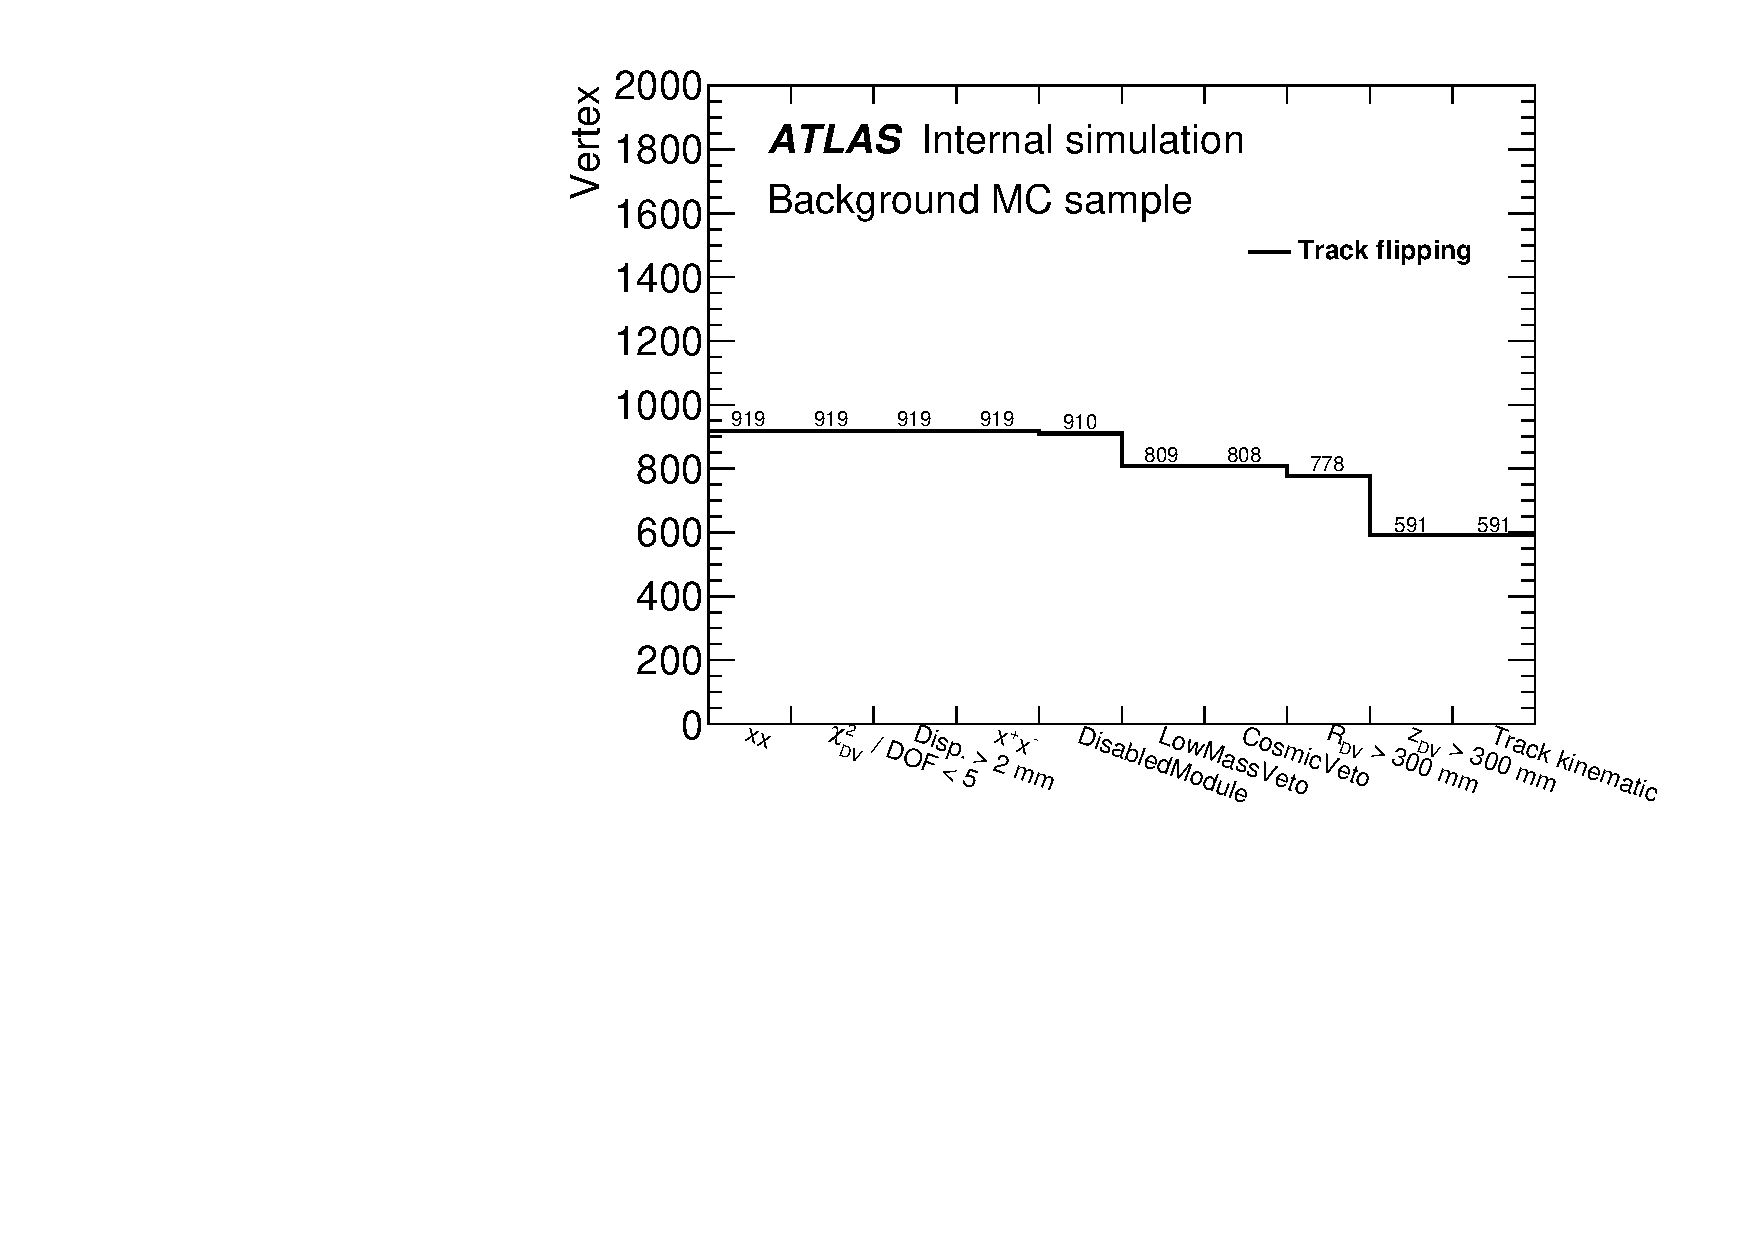
\includegraphics[width=0.60\textwidth]{figures/m_FBE_cutflow_MC.pdf}
	\centering
	\caption{Vertex cut flow applied on \xx vertices from the TF method.}
	\label{fig:m_FBE_cutflow_MC}
\end{figure}

The vertex yields from the TF and event mixing method, which represent the estimation for random-crossing background, are compared with the vertex yields from reconstruction in Table~\ref{table:random_vertex_count}. No random-crossing background of \mumu, \ee, or \emu type is expected from the MC samples using both methods. 
 
\begin{table}[!htb]
  \centering
  \begin{tabular}{ c  c c c }
    \hline
    \hline
	Vertex Type					& Track Flipping	        & Event Mixing	        & Background MC Samples \\
    \hline
	\mux						&	1						&	1.3 				&	0					\\
	\ex						    &	0						&	0.3 				&	0					\\
	\xx						    &	741 					&	714.0				&	676 				\\
    \hline
    \hline
  \end{tabular}
  \caption{Comparison of the number of \mux, \ex, and \xx vertices found in the track flipping, estimated from the event mixing, and reconstructed in the background MC samples.}
  \label{table:random_vertex_count}
\end{table}

The \xx vertex yields from the track flipping and the event mixing methods agree within the statistical uncertainty. The \xx vertex distributions of the vertices from the track flipping, event mixing, and from reconstruction are shown in Figure~\ref{fig:random-crossing_vertex_dist}. The distributions of the track flipping and the event mixing agree reasonably well with the distributions of vertices found from the reconstruction.

\begin{figure}[!htb]
    \centering
    \subfloat[]{\label{subfig:random-crossing_MC_M}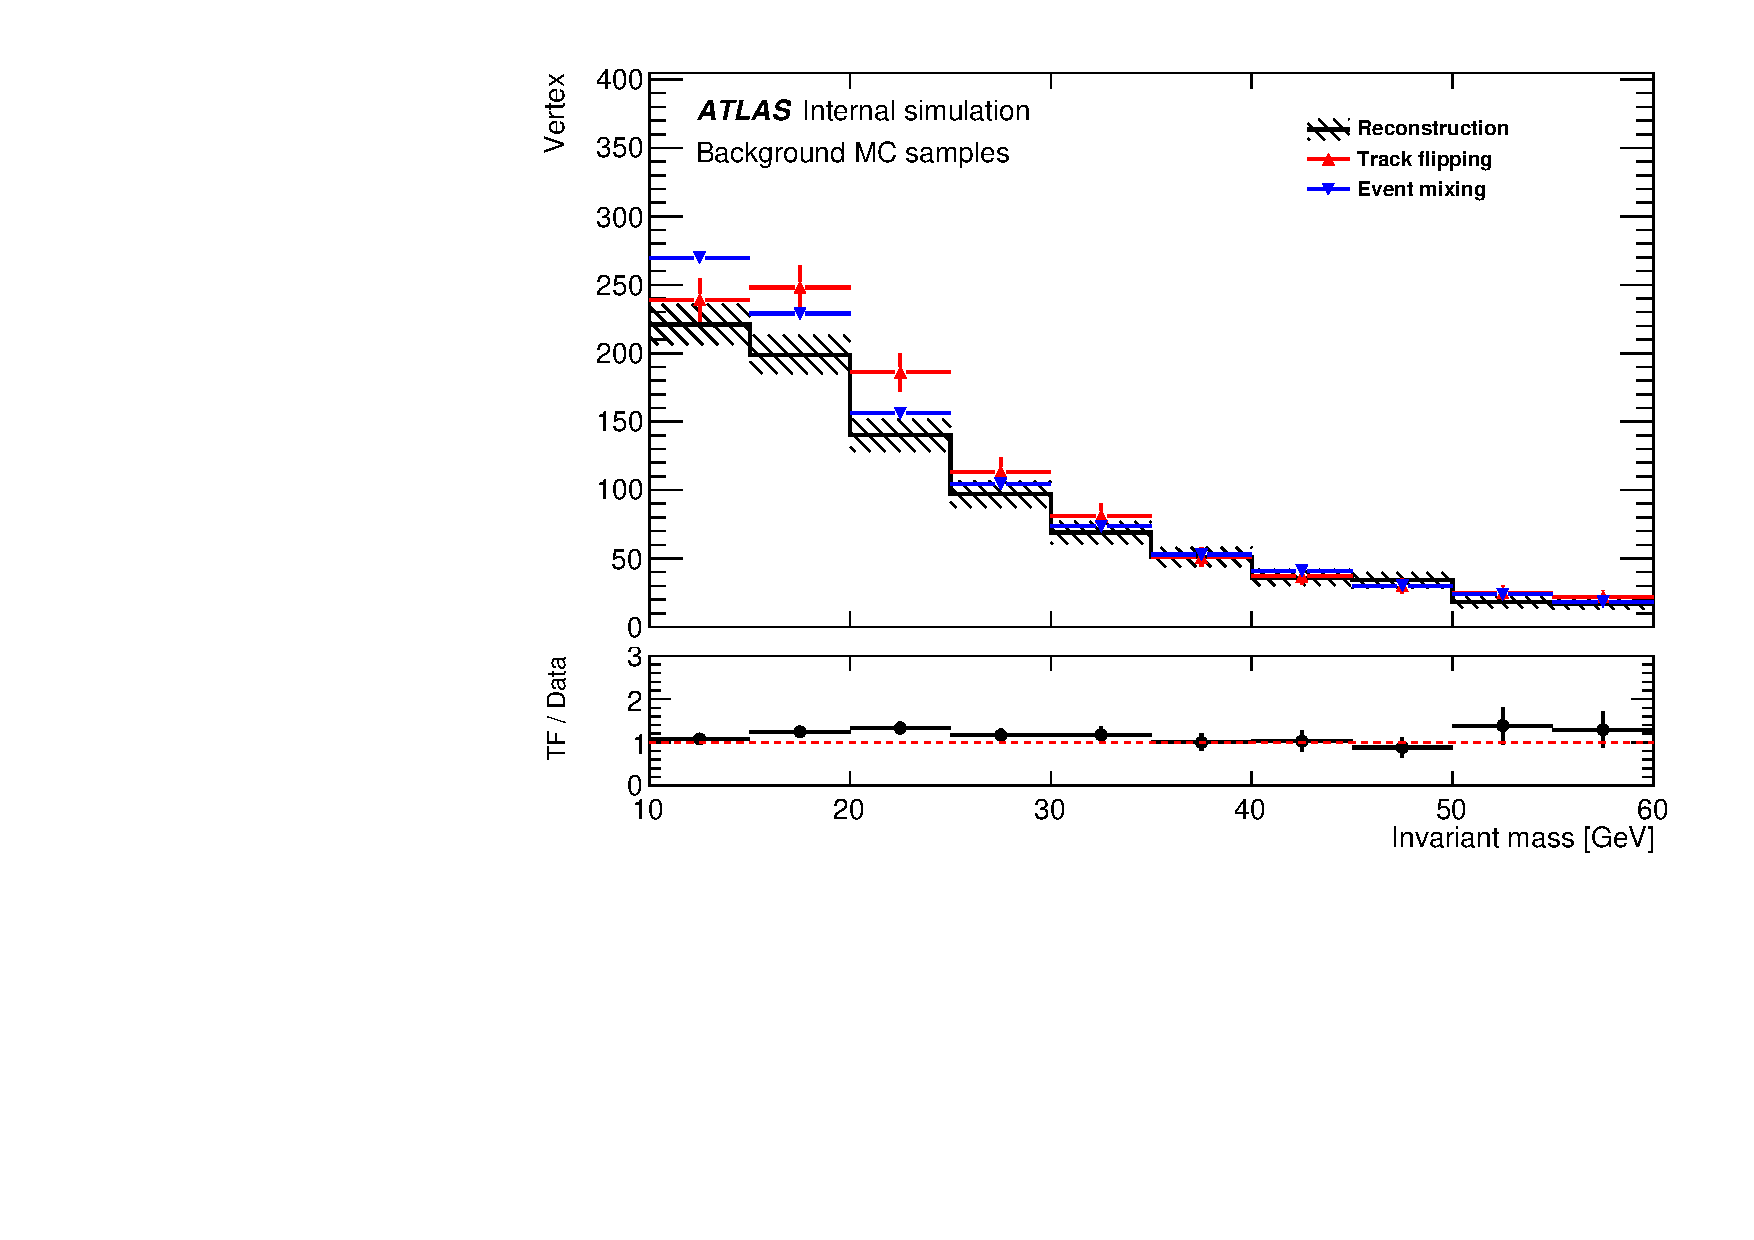
\includegraphics[width=0.45\textwidth]{figures/m_FBE_M.pdf}}
    \subfloat[]{\label{subfig:random-crossing_MC_chi2ndof}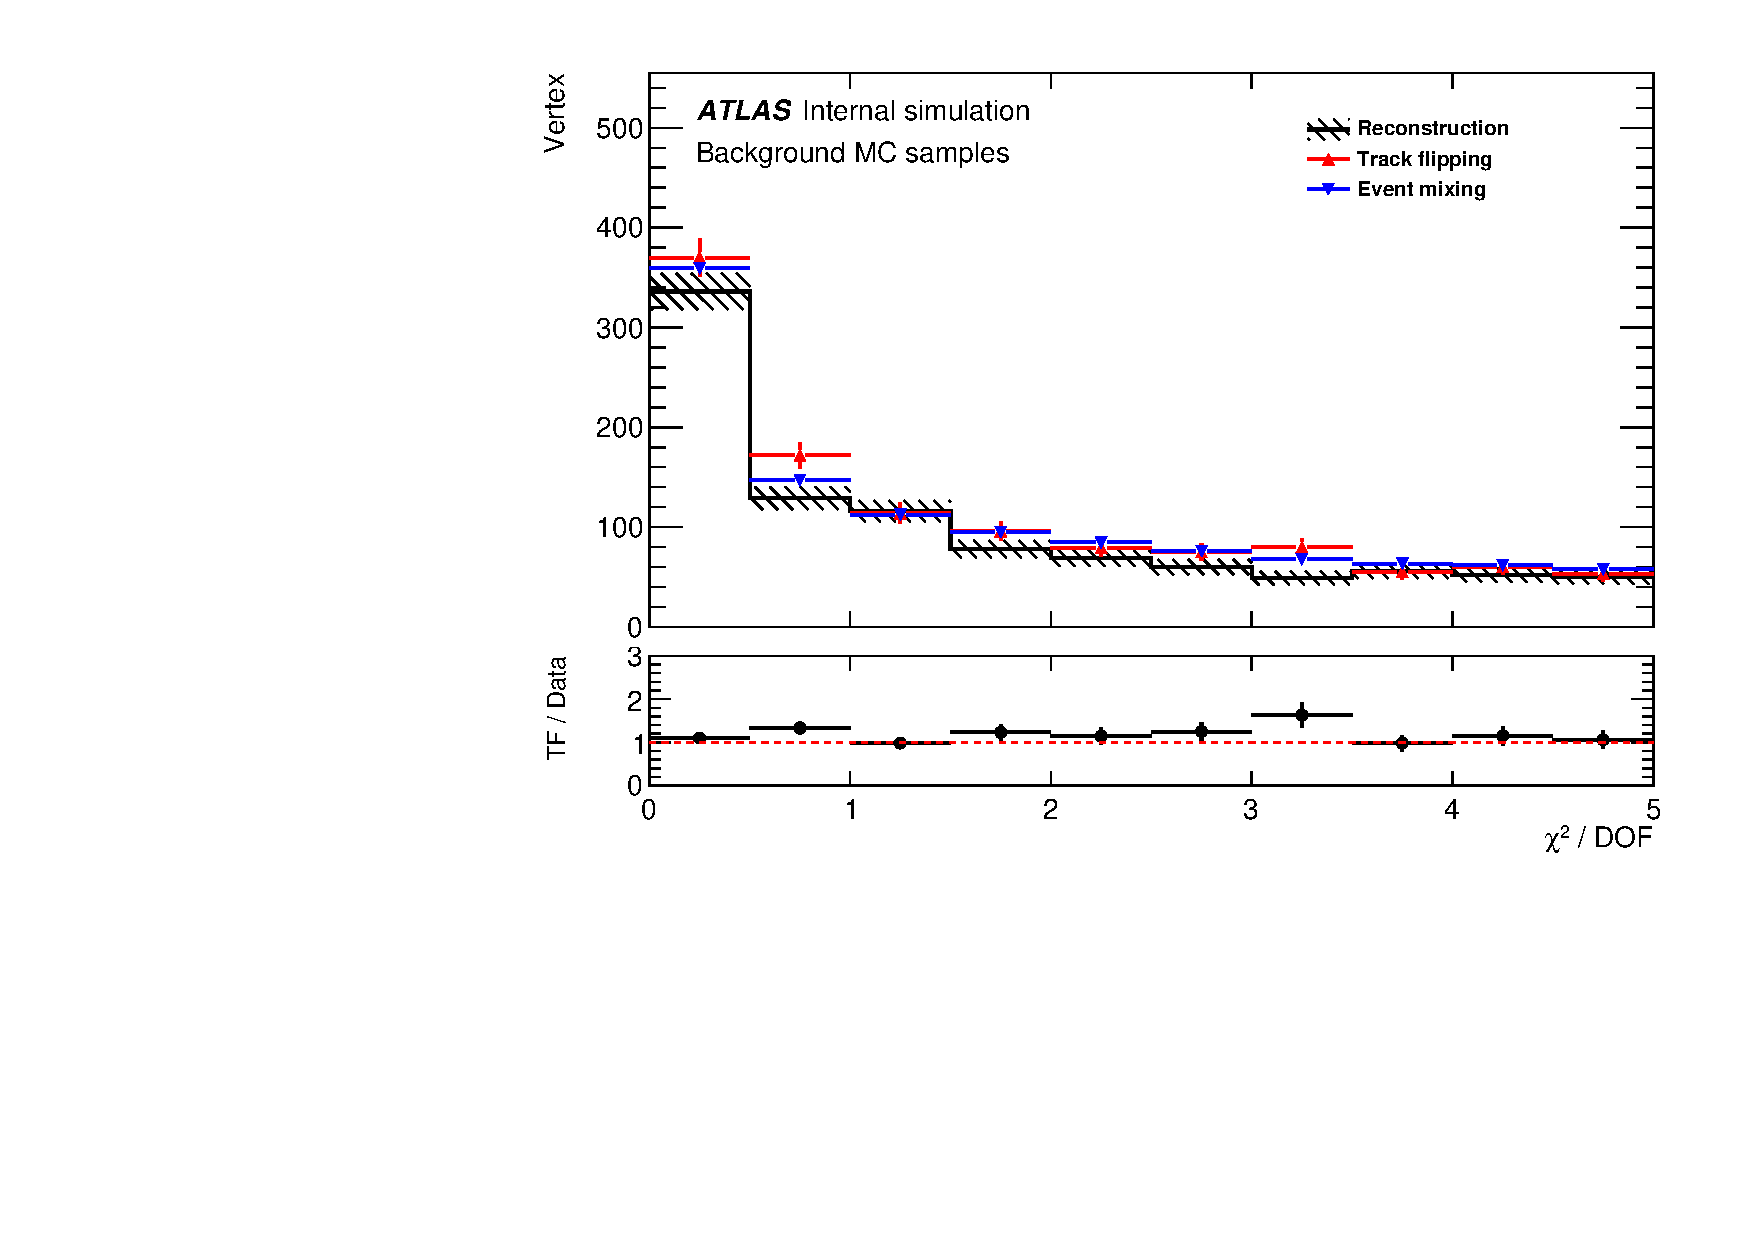
\includegraphics[width=0.45\textwidth]{figures/m_FBE_chi2_ndof.pdf}} \\
    \subfloat[]{\label{subfig:random-crossing_MC_r}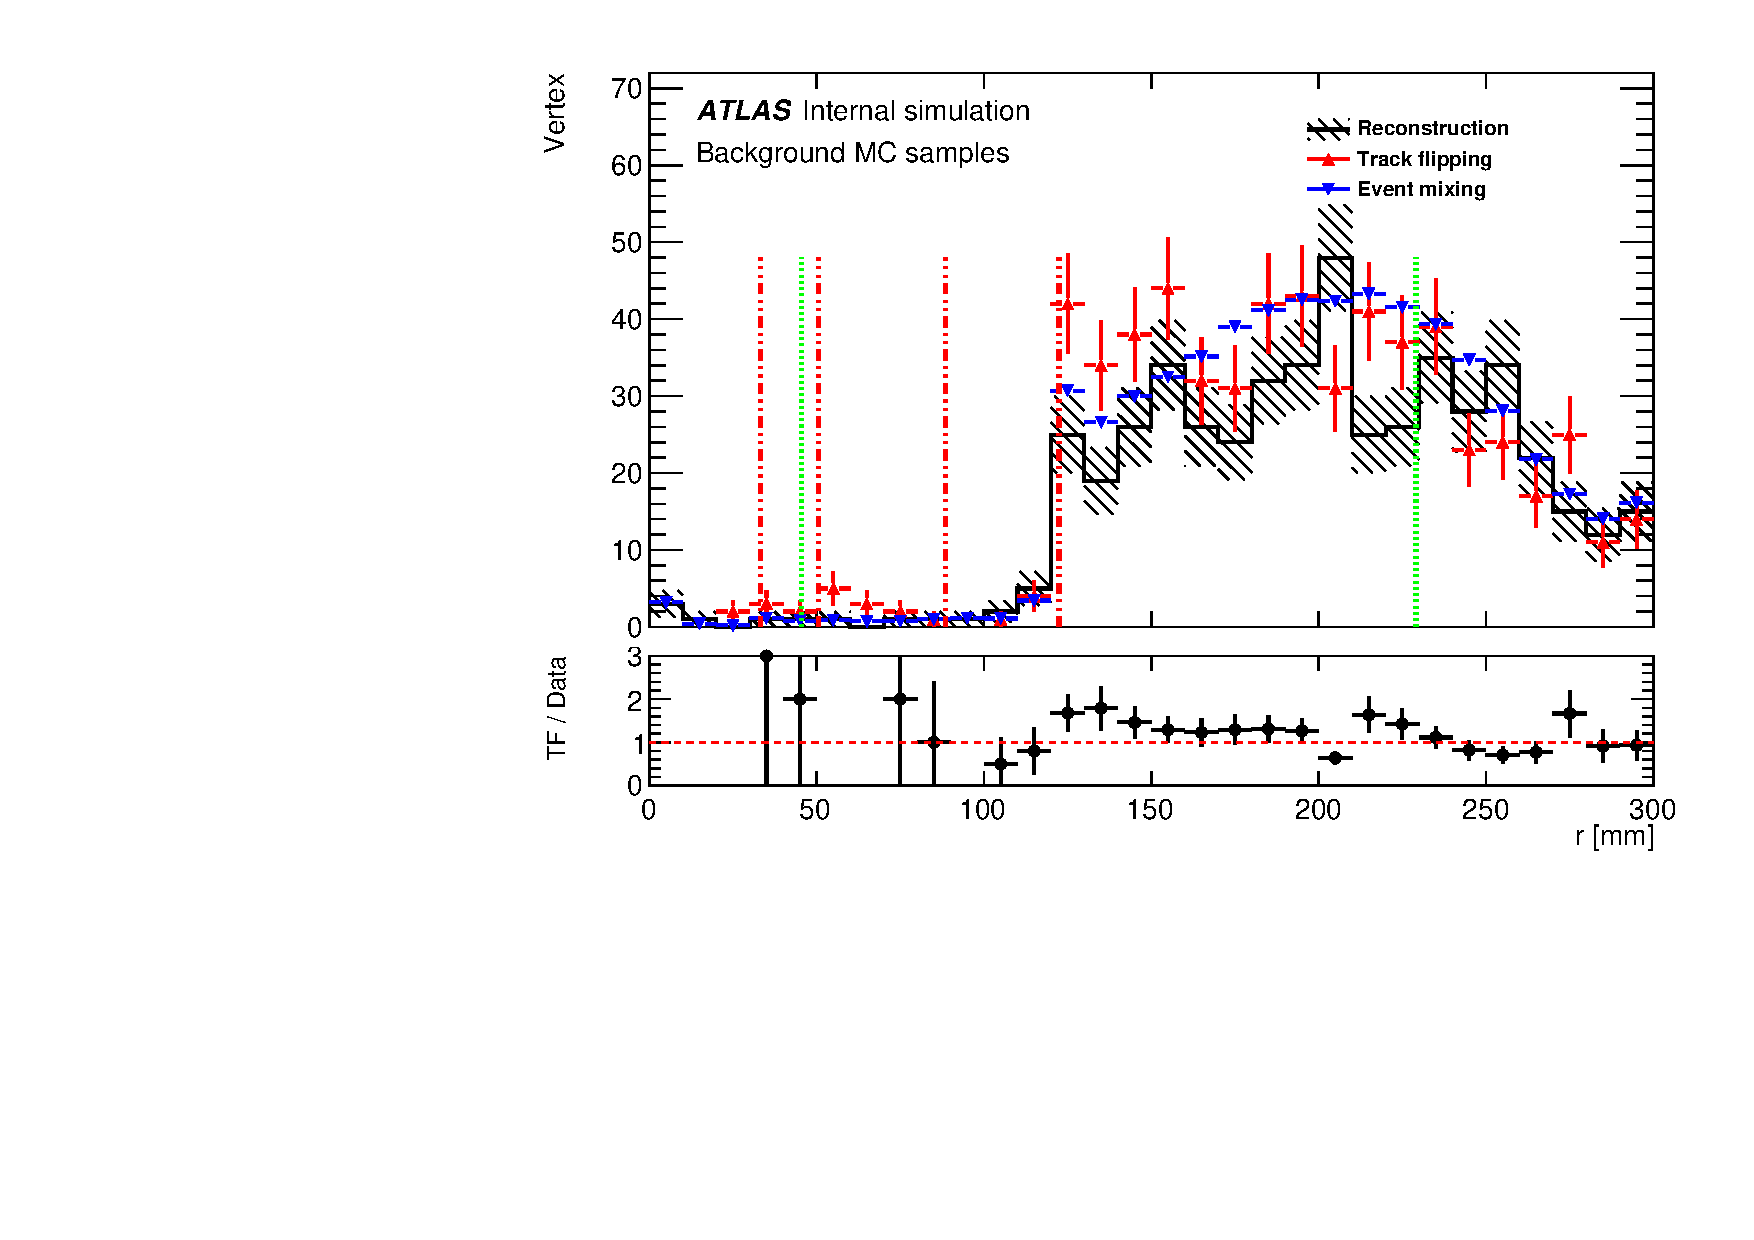
\includegraphics[width=0.45\textwidth]{figures/m_FBE_R.pdf}}
    \subfloat[]{\label{subfig:random-crossing_MC_z}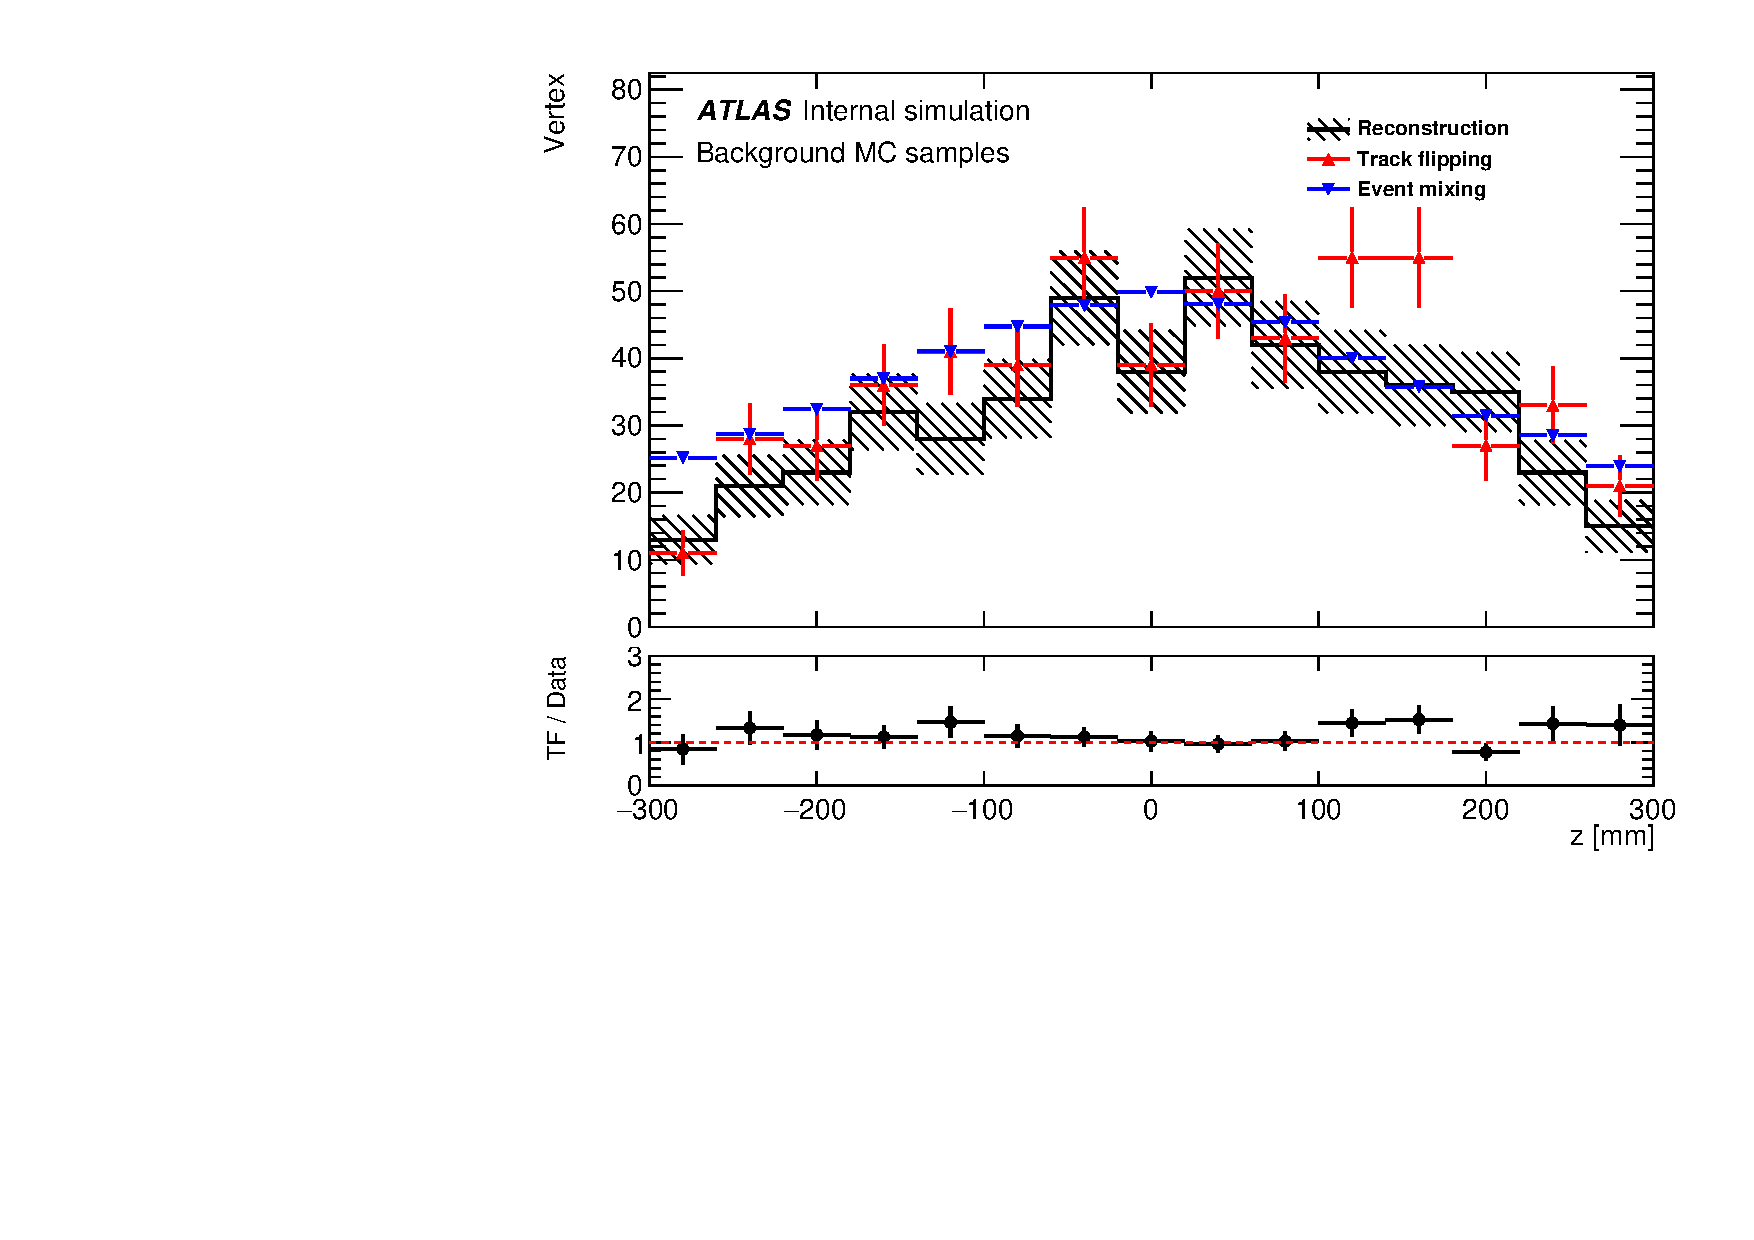
\includegraphics[width=0.45\textwidth]{figures/m_FBE_z.pdf}}
    %\subfloat[l]{\label{subfig:random-crossing_l}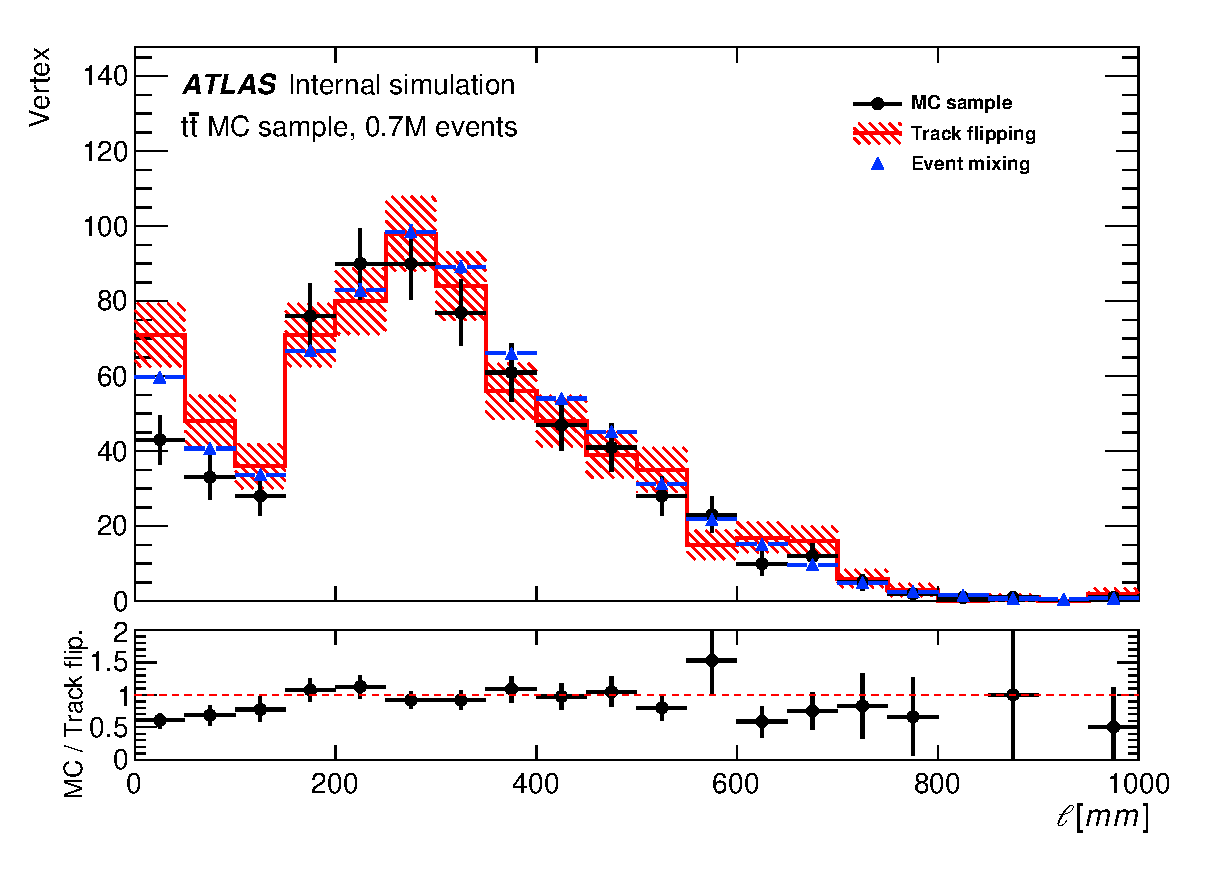
\includegraphics[width=0.45\textwidth]{figures/m_FBE_l.eps}}
    \caption{Comparison of of (a) vertex mass, (b) $\chi^{2} / \mathrm{DOF}$, (c) transverse, and (d) longitudinal position of \xx vertices reconstructed, found from the track flipping, and estimated using the event mixing. In (c), the red dashed lines indicate the four Pixel layers and the first layer of SCT. The green dotted lines indicate the Inner Support Tube (45.5 mm) and Pixel Support Tube (229 mm).}
    \label{fig:random-crossing_vertex_dist}
\end{figure}












\subsection{Estimating Random-crossing Background with Data Sample}
\label{sec:bkg:random_crossing_data}

Random-crossing background is estimated by performing the TF method on the data sample. Following the procedure described in Section~\ref{sec:bkg:random_crossing_tf}, track-flipping vertices are created, and the vertex yields in the control and validation regions are used to make an estimation in the signal region. 

\textbf{Vertex distribution in control region} In the control region, the \xx vertices found from the track flipping method are compared to the vertices reconstructed in the data sample in Figure~\ref{fig:random-crossing_vertex_dist_data}. The distributions shows that the TF method reproduces the data reasonably well including some of the structures of the ID, suggesting that the TF method provides a reasonable estimation of the random-crossing background.

\begin{figure}[!htb]
    \centering
    \subfloat[]{\label{subfig:random-crossing_M}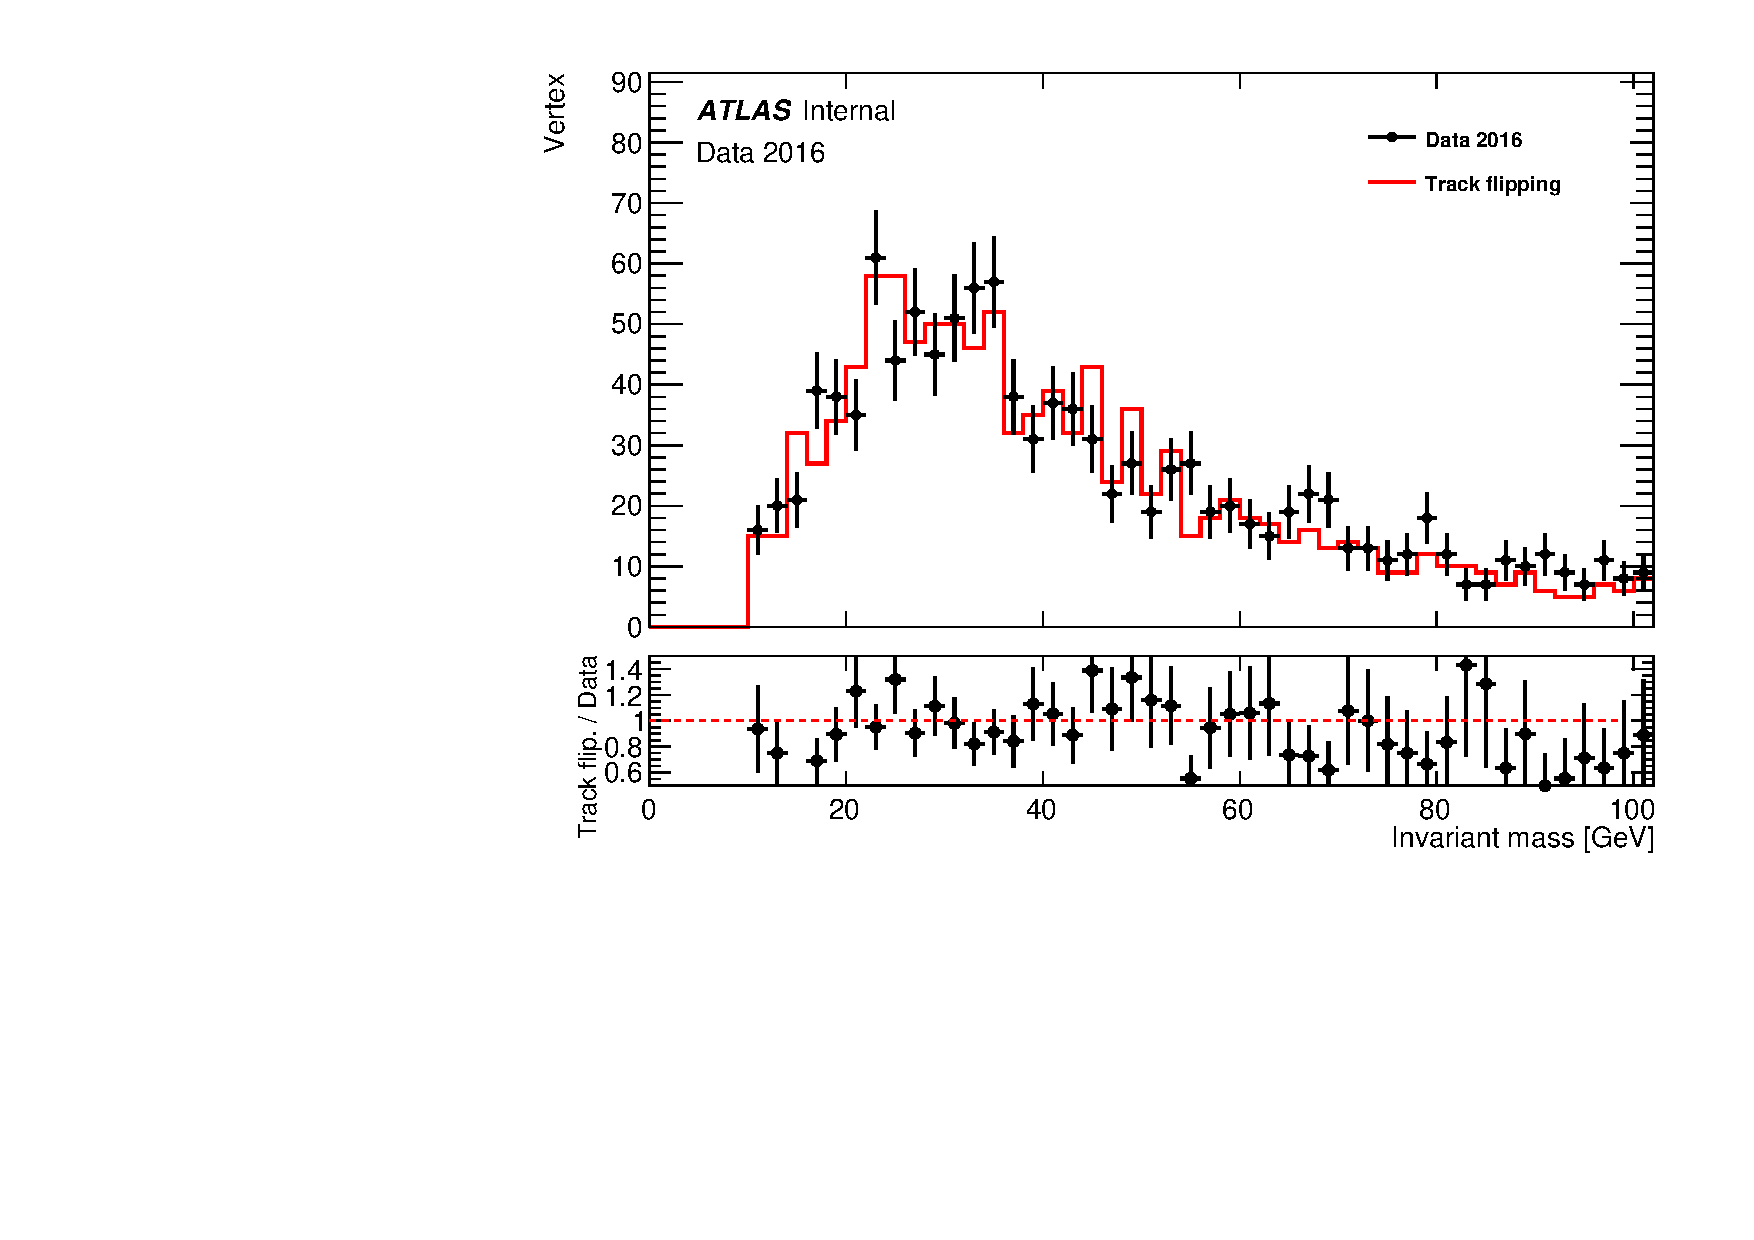
\includegraphics[width=0.45\textwidth]{figures/m_FBE_data_M.pdf}}
    \subfloat[]{\label{subfig:random-crossing_chi2ndof}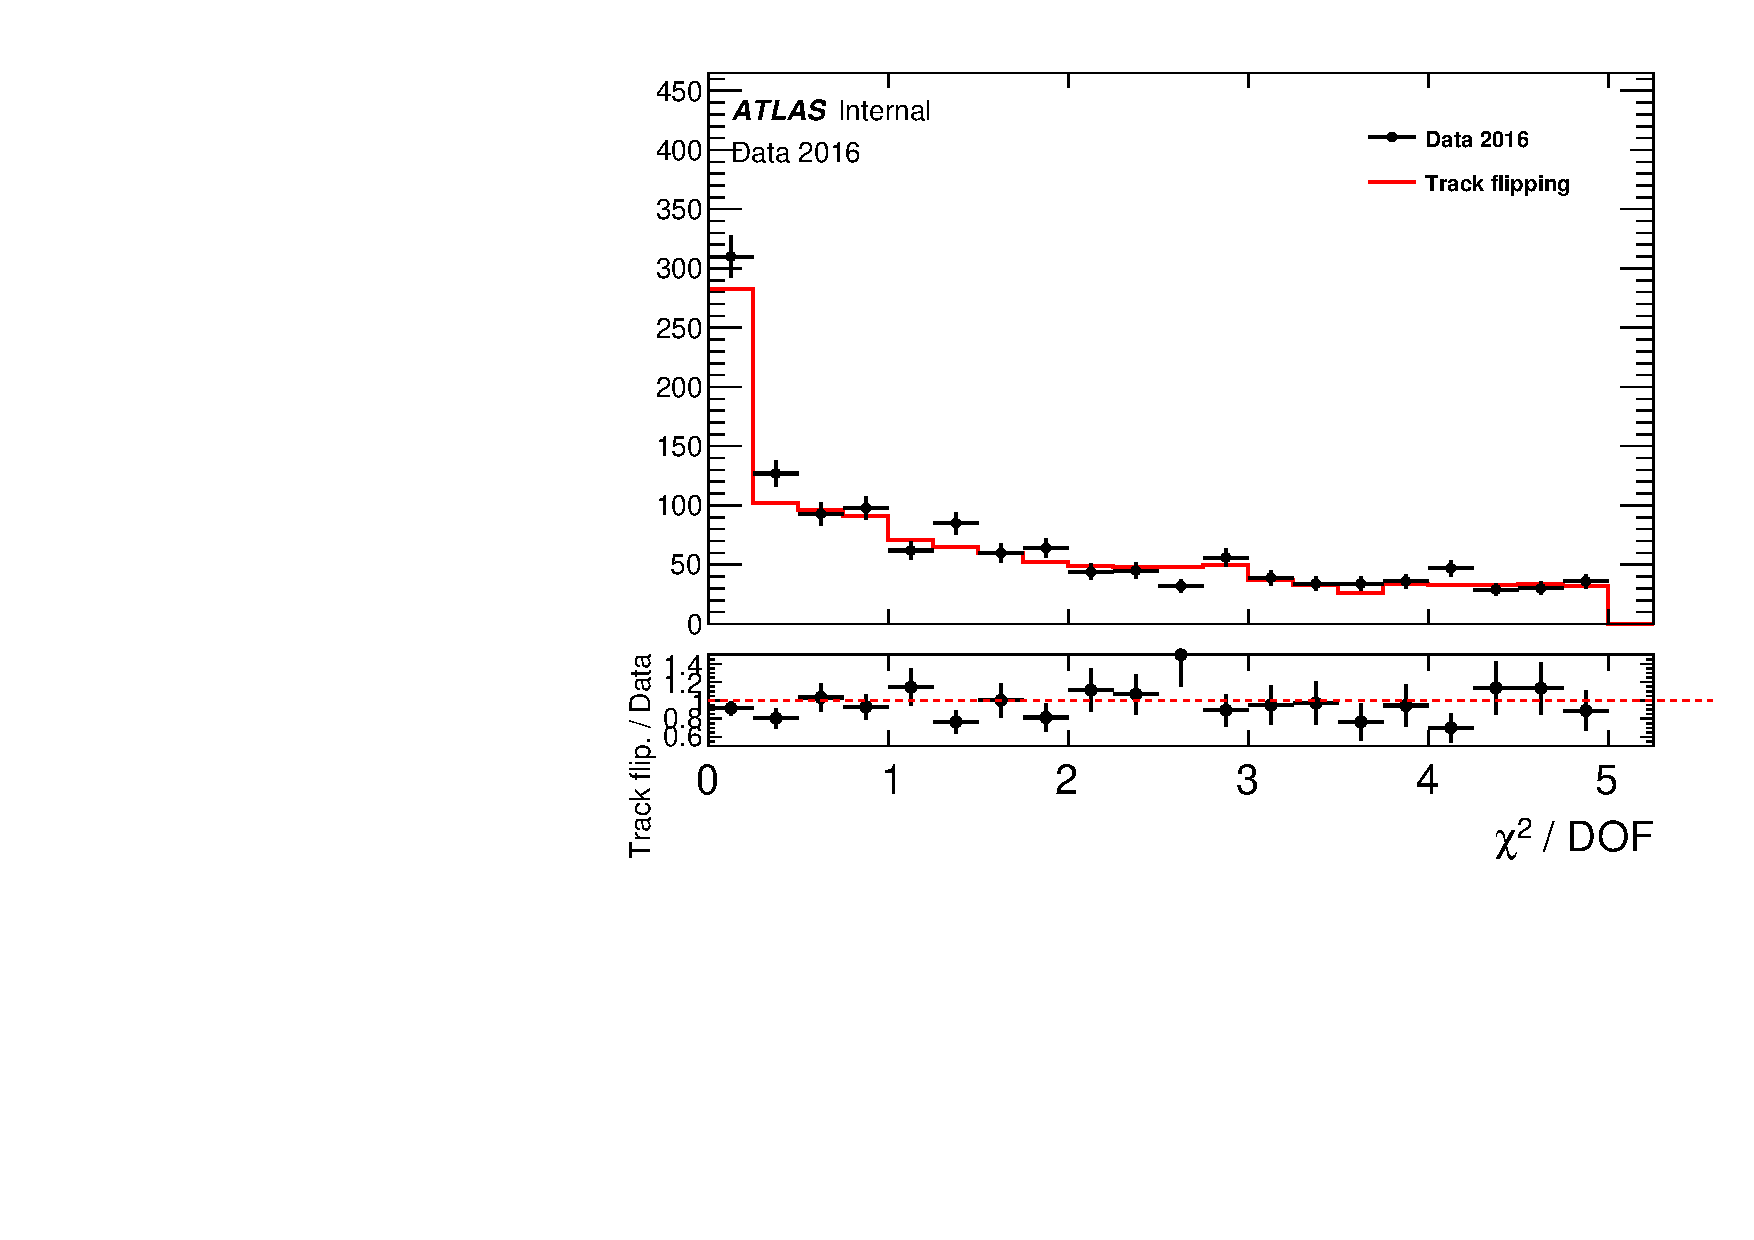
\includegraphics[width=0.45\textwidth]{figures/m_FBE_data_chi2_ndof.pdf}} \\
    \subfloat[]{\label{subfig:random-crossing_r}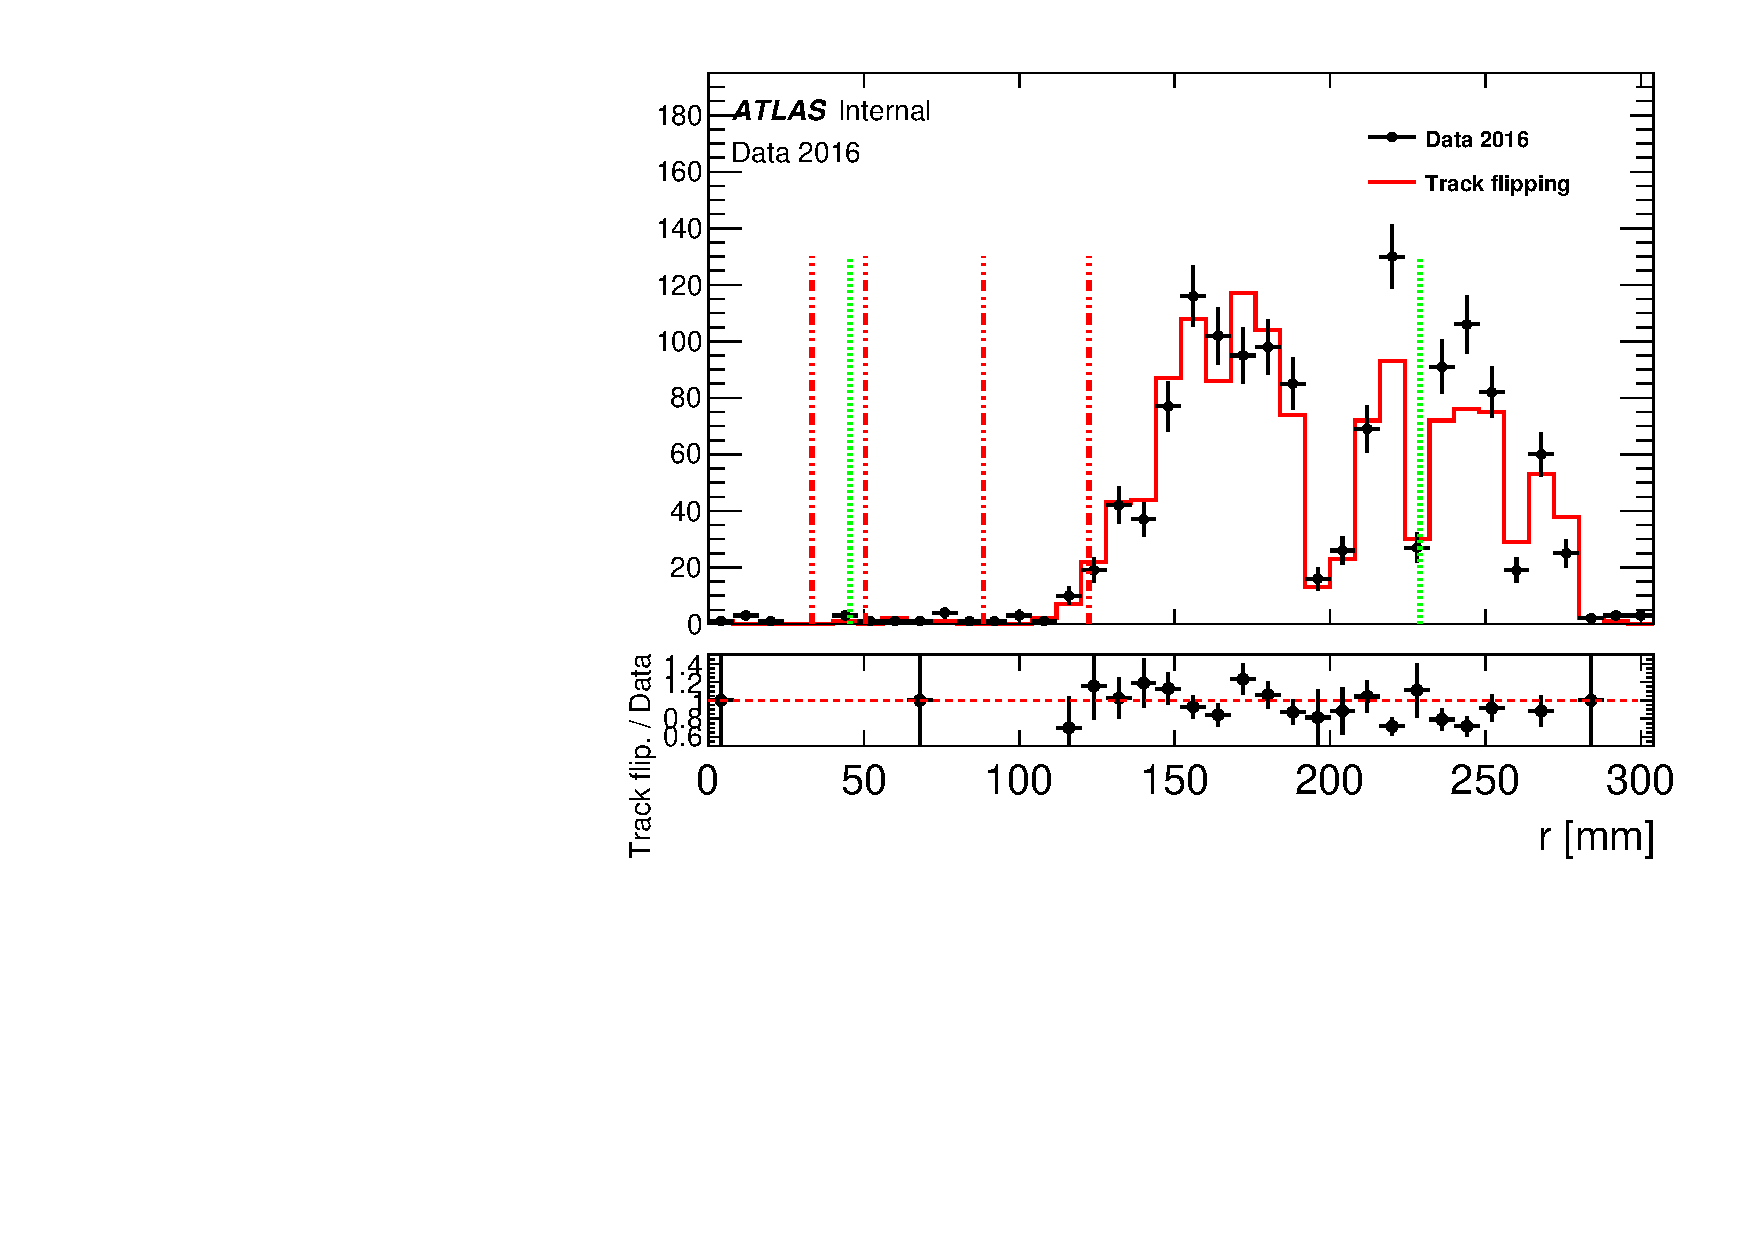
\includegraphics[width=0.45\textwidth]{figures/m_FBE_data_R.pdf}}
    \subfloat[]{\label{subfig:random-crossing_z}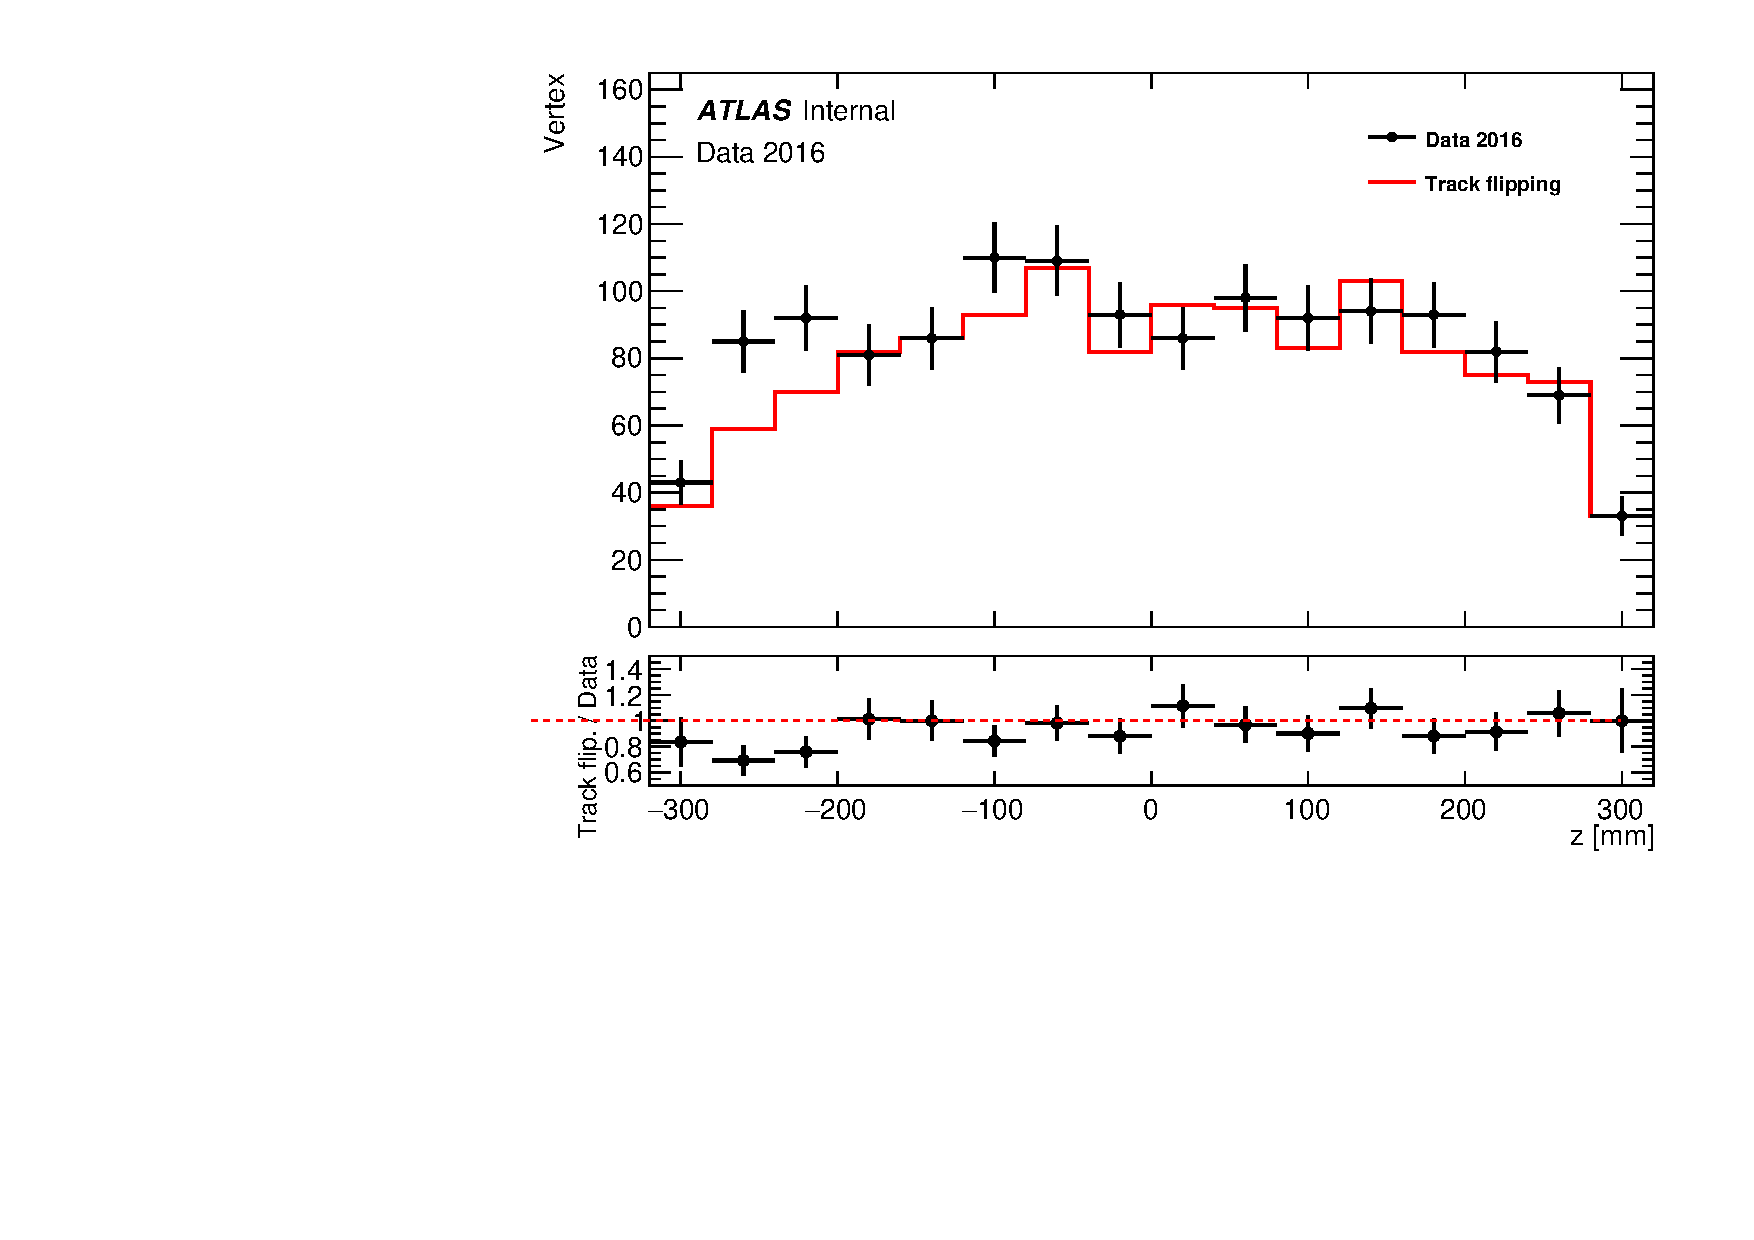
\includegraphics[width=0.45\textwidth]{figures/m_FBE_data_z.pdf}}
    %\subfloat[l]{\label{subfig:random-crossing_l}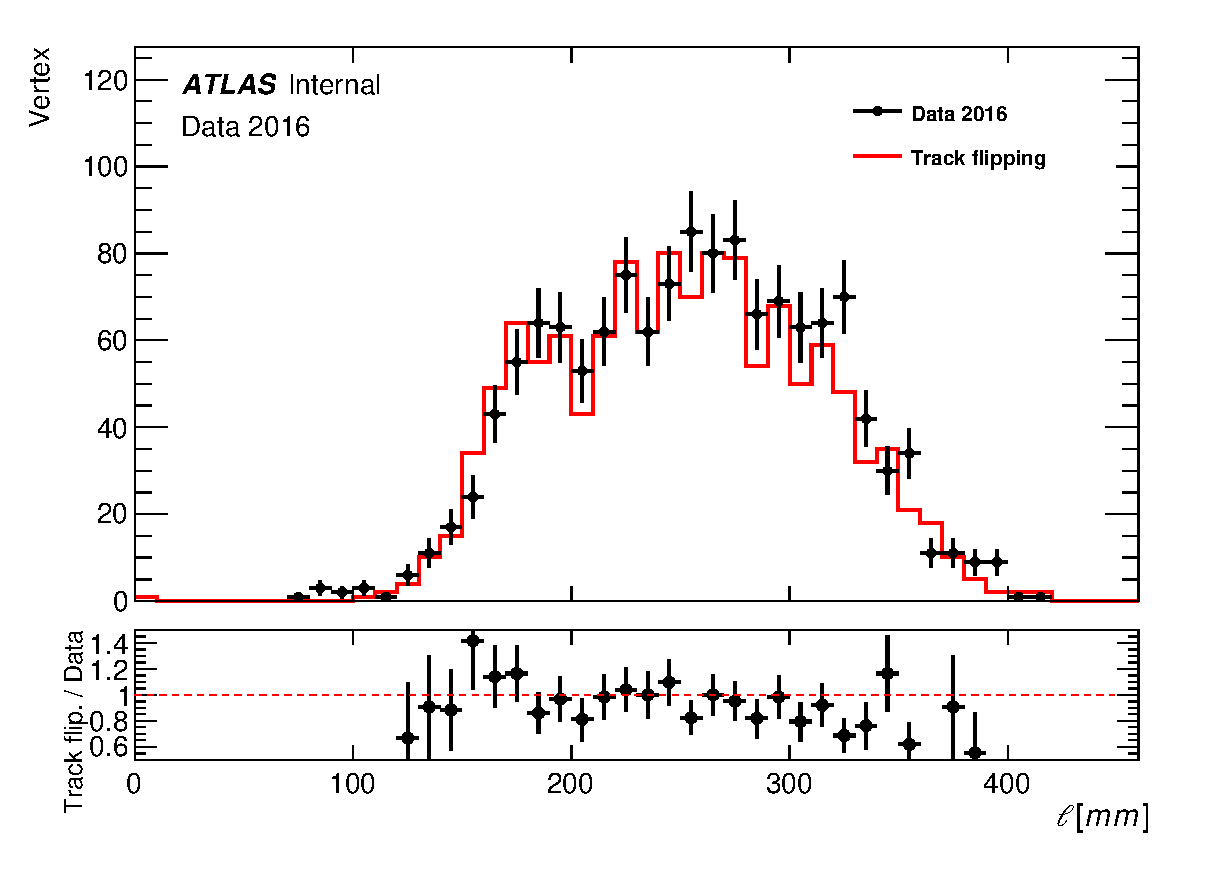
\includegraphics[width=0.45\textwidth]{figures/m_FBE_data_l.eps}}
    \caption{Comparison of (a) vertex mass, (b) $\chi^{2} / \mathrm{DOF}$, (c) transverse, and (d) longitudinal position of vertices found from reconstruction with the track-flipping vertices in the control region of the data sample. In (c), the red dashed lines indicate the four Pixel layers and the first layer of SCT. The green dotted lines indicate the Inner Support Tube (45.5 mm) and Pixel Support Tube (229 mm).}
    \label{fig:random-crossing_vertex_dist_data}
\end{figure}

However, because of the limited statistics in lepton pairs in the data sample, the track-flipping vertex yields in the signal region cannot be directly used as random-crossing background estimation. Instead, the track-flipping vertex yields in the control region and validation region are extrapolated to estimate random-crossing background in the signal region using lepton probability, defined as follows:
\begin{itemize}
\item $P(e)$ is defined as the ratio of electrons to inner detector tracks in the entire sample,
\item $P(\mu)$ is defined as the ratio of muons to inner detector tracks in the entire sample,
\end{itemize}
where track requirements described in Table~\ref{table:vertex_track_selection_simple} is required to both leptons and inner detector tracks.

\textbf{Extrapolation from control region} The track-flipping vertex yields in the control region is extrapolated using Eq.~\ref{eq:TF_extrapolation_from_control} to the validation regions to estimate the vertex yields, representing random-crossing background estimation in the validation region. The estimated \mux and \ex vertex yields are compared with the observed track-flipping vertex yield in the region. The ratio of the observed track-flipping vertex to the extrapolated vertex in the validation region is used as scale factors for the estimation in the signal region,

\begin{align}
    %S_{xx\rightarrow \mu x} &= N_{\mu x}^{obs} / N_{\mu x}^{est}, \nonumber \\
    %S_{xx\rightarrow \ex}   &= N_{e x}^{obs} / N_{e x}^{est}
    S_{xx\rightarrow \mu x} &= \frac{N_{\mu x}^{obs}}{N_{\mu x}^{est}}, \nonumber \\
    S_{xx\rightarrow \ex}   &= \frac{N_{e x}^{obs}}{ N_{e x}^{est}}
\label{eq:random_crossing_scale_factor}
\end{align}
where $N_{\mu x}^{obs}$ and $N_{\mu x}^{est}$ ($N_{ex}^{obs}$ and $N_{ex}^{est}$) represent the number of observed track-flipping vertex and the estimated vertex of each type.

The track-flipping vertex yield is then extrapolated to the signal region using Eq.~\ref{eq:TF_extrapolation_from_control} to estimate random-crossing background, and the scale factors defined by Eq.~\ref{eq:TF_scale_factors} are applied to the extrapolation for more accurate estimation of the background.

\textbf{Extrapolation from validation region} Similarly, the track-flipping vertex yields in the validation region is extrapolated to the signal to estimate vertex yields using Eq.~\ref{eq:TF_extrapolation_from_validation}, and the scale factors defined by Eq.~\ref{eq:TF_scale_factors} are applied to the extrapolation to obtain the background estimation.

The lepton probability, track-flipping and reconstructed vertex yields in the control and validation region, the scale factors, and the estimated random-crossing background are summarized in Table~\ref{table:track_flipping}.

\begin{table}[!htb]%
  \centering
  \begin{minipage}[b]{\textwidth}
  \resizebox{\textwidth}{!}{
  \subfloat[Lepton probability]{
    \begin{tabular}[t]{ccc}
        \hline\hline
                & Tracks             & p($\ell$)           \\
         \hline
         x      & $2.47\times10^{7}$ & -                   \\
         $\mu$  & $5.23\times10^{4}$ & $2.10\times10^{-3}$ \\
         $e$    & $3.63\times10^{4}$ & $1.46\times10^{-3}$ \\
         Sum    & $2.48\times10^{7}$ & - \\
        \hline\hline
    \end{tabular}
  }
  \qquad
  \subfloat[Vertex yields in the control and validation region]{
    \begin{tabular}[t]{ccc}
        \hline\hline
                & Tracks-flipping    & Data                \\
         \hline
         $xx$   & 1255               & 1346                \\
         $\mu x$& 3                  & 4                   \\
         $ex$   & 1                  & 0                   \\
        \hline\hline
    \end{tabular}
  }%
  \qquad
  \subfloat[Scale factors]{
    \begin{tabular}[t]{cc}
        \hline\hline
         Type                      & SF      \\
         \hline
         $S_{xx\rightarrow\mu x}$  & 0.82              \\
         $S_{xx\rightarrow ex}$    & 0.19              \\
        \hline\hline
    \end{tabular}
  }
  }
  \end{minipage}


  \subfloat[Extrapolation from control region]{
    \begin{tabular}[t]{ccc}
        \hline\hline
                         & Estimation          & Applying SF         \\
         \hline
         $N_{\mu x}$     & 4                   & -                   \\
         $N_{e x}$       & 5                   & -                   \\
         $N_{\mu\mu}$    & $2.69\times10^{-3}$ & $1.79\times10^{-3}$ \\
         $N_{ee}$        & $5.56\times10^{-3}$ & $1.99\times10^{-4}$ \\
         $N_{e\mu}$      & $7.73\times10^{-3}$ & $1.96\times10^{-3}$ \\
        \hline\hline
    \end{tabular}
  }%
  \qquad
  \subfloat[Extrapolation from validation region]{
    \begin{tabular}[t]{ccc}
        \hline\hline
                         & Estimation          & Applying SF         \\
         \hline
         $N_{\mu\mu}$    & $2.19\times10^{-3}$ & $1.79\times10^{-3}$ \\
         $N_{ee}$        & $1.05\times10^{-3}$ & $1.99\times10^{-4}$ \\
         $N_{e\mu}$      & $3.89\times10^{-3}$ & $1.96\times10^{-3}$ \\
        \hline\hline
    \end{tabular}
  }%
  %}
  
  \caption{Random-crossing background estimation in data by the TF method}%
  \label{table:track_flipping}
\end{table}


%The systematic uncertainty in the track flipping method is estimated by studying the variance in background estimation from different variations of the track flipping method. In addition to the transformation described in the previous section ($d_{0}\rightarrow -d_{0}, z_{0}\rightarrow -z_{0}, \phi\rightarrow\phi-\pi, \theta\rightarrow\pi-\theta$), the following track transformations are considered.
%\begin{itemize}
%\item \textbf{Same sign d0}: $d_{0}\rightarrow d_{0}, z_{0}\rightarrow -z_{0}, \phi\rightarrow\phi-\pi, \theta\rightarrow\pi-\theta$
%\item \textbf{Same sign $\theta$}: $d_{0}\rightarrow -d_{0}, z_{0}\rightarrow -z_{0}, \phi\rightarrow\phi-\pi, \theta\rightarrow\theta$
%\item \textbf{90 degrees rotation in $\phi$}: $d_{0}\rightarrow -d_{0}, z_{0}\rightarrow -z_{0}, \phi\rightarrow\phi-\frac{\pi}{2}, \theta\rightarrow\theta$
%\end{itemize}

%\subsection{Systematic uncertainty in random-crossing background}
%\label{sec:bkg:random_crossing_syst}
